%% New template changes

\documentclass[a4paper,10pt,oneside,onecolumn,final,openright]{report}
\usepackage{helvet} %Arial-like font
\renewcommand{\familydefault}{\sfdefault} %Apply helvet font
\usepackage[margin=2.5cm]{geometry} %Apply 2.5cm margin in all sides

\usepackage[doublespace,indent]{thesisdavid} %Change chapter style or font / line spacing in thesisdavid.sty
%%%%%%%%%%%%%%%%%%%%%%%%%%%%%%%%%%%%%%%%%%%%%%%%%%%%%%%%%%%%%%%%%%%%%%%%

\usepackage[utf8]{inputenc}
\usepackage[english]{babel}
\usepackage{url}

\usepackage{array,booktabs,arydshln}
\usepackage{hyphenat}
\usepackage{graphicx}
\usepackage{flushend}
\usepackage{caption}
\usepackage{subfig}
\usepackage{algpseudocode}
\usepackage{algorithm}
\usepackage{amsmath}
\usepackage{amssymb}
\usepackage{afterpage}
\usepackage[explicit]{titlesec}
\usepackage[acronym]{glossaries}

\makeglossaries

\newcolumntype{M}[1]{>{\centering\arraybackslash}m{#1}}

\newcommand{\red}[1]{\textcolor{red}{#1}}
\newcommand{\todo}[1]{\textcolor{red}{\{TODO:} #1\textcolor{red}\}}

\definecolor{light}{gray}{.85}

\algdef{SE}[VARIABLES]{Variables}{EndVariables}
   {\algorithmicvariables}
   {\algorithmicend\ \algorithmicvariables}
\algnewcommand{\algorithmicvariables}{\textbf{global variables}}


\begin{document}
%\nocite{*}  %Show bibliography without explicit citations

% Initial pages.
\thispagestyle{empty}

\begin{singlespace}
\vbox to\textheight{%
%--------------------------------------------------
%\vskip-1.3in%---------- LOGO E NOME IST/UTL -------
%--------------------------------------------------
%\hskip-17mm
\vbox to50mm{
%\vfil
\begin{tabular}{l}

\includegraphics[width=5cm]{figs/Logo_IST_web.pdf}
\end{tabular}
\vfil
\vfil
}%
%--------------------------------------------------
\vskip6mm%---------- TTULO -----------------------
%--------------------------------------------------
\vbox to25mm{\LARGE\bf
\vfil
\begin{center}
Adaptive Information Dissemination in the Bitcoin Network
\end{center}
\vfil
}%
%--------------------------------------------------
\vskip10mm%---------- NOME E GRAU ACTUAL -----------
%--------------------------------------------------
\vbox to25mm{\large
\vfil
\begin{center}
{\Large\bf João Esteves Marçal}\\   % author's name
\end{center}
\vfil
}%
%--------------------------------------------------
\vskip10mm%---------- GRAU A OBTER -----------------

%--------------------------------------------------
\vbox to8mm{\large
\vfil
\centerline{Thesis to obtain the Master of Science Degree in}
\vskip3mm
\centerline{{\bf \LARGE Information Systems and Computer Engineering}}
\vfil
\vskip15mm

\begin{center}
Supervisors:\\
Prof. Lu\'{i}s Eduardo Teixeira Rodrigues\\
Prof. Miguel Ângelo Marques de Matos\\
\end{center}

}%
% %--------------------------------------------------
\vskip45mm %---------- JURI -------------------------
% %--------------------------------------------------
\vbox to7mm{\bf
\vfil
\begin{center}
{\bf \Large Examination Committee}\\
\end{center}
\vfil
}%


\vbox to28mm{
\vfil
{\large
\begin{center}
\begin{tabular}{p{0.35\textwidth}l}
Chairperson: &  Prof. "To Be Defined" \\
%Advisor: & Prof. Doutor Lu\'{i}s Eduardo Teixeira Rodrigues\\
Supervisor: & Prof. Miguel Ângelo Marques de Matos\\
Member of the Committee: & Prof. João Carlos Antunes Leitão \\
\end{tabular}
\end{center}
}
\vfil
}%
%--------------------------------------------------
\vskip28mm%---------- DATA -------------------------
%--------------------------------------------------
\vbox to4mm{\Large\bf
\vfil
\begin{center}
October 2018
\end{center}
\vfil
}%
%--------------------------------------------------
}%vbox
\end{singlespace}
\null\newpage

\pagestyle{plain}

\chapter*{Acknowledgements}
I would like to thank my advisors Professor Miguel Matos and Professor Luís Rodrigues, for their guidance throughout this work. 
I would also like to thank my friends for all the leisure moments we shared during this year. 
Last, but definitely not least, I would like to thank my parents and my sisters for the endless support.
\\
\\
\\
\\
This work was partially supported by Fundo Europeu de Desenvolvimento Regional (FEDER) through Programa Operacional Regional de Lisboa and by Fundação para a Ciência e Tecnologia (FCT) through projects with reference UID/CEC/50021/2013 and LISBOA-01-0145-FEDER- 031456.
\chapter*{Resumo}
Gostava de agradecer a

\null\newpage
\chapter*{Abstract}
Gostava de agradecer a

\null\newpage

\chapter*{Palavras Chave\\Keywords}

\section*{Palavras Chave}

Livro Razão

Criptomoeda

Disseminação de informação

Adaptablidade

Utilização de recursos

\section*{Keywords}

Ledger

Cryptocurrency

Information dissemination

Adaptation

Resource Usage
\tableofcontents
\listoffigures
\newacronym{pow}{PoW}{Proof of Work}

\newacronym{lcm}{LCM}{Least Common Multiple}

\newacronym{p2p}{P2P}{Peer to Peer}

\newacronym{ip}{Ip}{Initial push}


\printglossary[type=\acronymtype]

\null\newpage

\chapter{Introduction}
Cryptocurrencies like Bitcoin and others gained a lot of exposure in the previous year, which has led to their popularization with an increase in average daily users. As a consequence of this increase, there has also been an increase in the resources spent by cryptocurrencies.

This thesis addresses two problems, the immense amount of resources spent on disseminating information and BLANK (MEMBERSHIP). In particular, we propose a new algorithm for the dissemination of transactions as well as an improvement in the current BLANK (MEMBERSHIP)
\section{Motivation}
Cryptocurrencies and their associated mechanisms have gained an increasing relevance in recent years. For instance, at the time of this writing, Bitcoin (the most widely used cryptocurrency) has peaked at a trading value of more than 20K USD and the Bitcoin network processed more than 250K transactions per day\footnote{Taken from \url{https://blockchain.info/charts}.}. Moreover, the main technology behind Bitcoin, the Blockchain, has emerged as useful for a myriad of other applications, from birth, wedding, and death certificates to the monetization of music\footnote{Taken from \url{https://blockgeeks.com/guides/blockchain-applications/}}.

For instance in Bitcoin, in an attack known as the partition attack,  an Autonomous System (AS) can isolate a partition of the network to make it vulnerable to double spending (see~\cite{apostolaki2016hijacking}).
Attacks such as this are increasingly more appealing due to the significant financial advantage that an attacker can gain, if successful.
It is therefore of the utmost importance to the future of cryptocurrencies to design mechanisms that eliminate, or at least mitigate the possibility of such attacks without sacrificing other important aspects of cryptocurrencies.

We are particularly interested in studying the protocols that support information dissemination in blockchain networks, and their vulnerabilities, as these are the backbone that allows cryptocurrencies to function properly.
Even though cryptocurrencies have attracted lots of attention from the community on higher level subjects such as the consensus protocol used, few works explore the subject of information dissemination~\cite{miller2015discovering, heilman2015eclipse, bojja2017dandelion, owenson2017proximity}.
%Strikingly, the few that do, show that information dissemination in cryptocurrencies is brittle and can have a severe impact on the system~\cite{miller2015discovering}.

\todo{Check from here}
In this work, we aim to address this problem by: i) doing a principled analysis of information dissemination vulnerabilities in the Bitcoin network and ii) proposing an extensible architecture that eliminates or mitigates these vulnerabilities.
We consider attackers with varying resources, from a rogue Autonomous System to a set of colluding individuals that target a specific victim, and different motivations in the system.
To address these, we look at techniques that have been proposed in distributed systems literature such as overlay networks~\cite{jesi2009secure} or node behaviour~\cite{li2006bar}.

Leveraging these techniques, we propose BitShield, an extensible architecture that aims to harden information propagation in cryptocurrency networks. More precisely, we focus on Bitcoin, but as we will see later the approach can be applied to other cryptocurrencies as well. The reason for choosing Bitcoin is that it is the most popular cryptocurrency and its core design is shared by many other cryptocurrencies, hence improvements over Bitcoin could be easily applied in other systems.

A maioria das criptomodedas existentes, e em particular a \emph{Bitcoin} (a criptomoeda mais usada correntemente), mantêm um livro-razão descentralizado que regista a sequência ordenada de todas as transacções executadas no sistema~\cite{nakamoto2008bitcoin}.
A manutenção de um livro-razão de forma descentralizada e aberta tem vindo a ser reconhecida como uma abstracção útil para várias aplicações, para além do uso original como meio de pagamento.
Por exemplo,  livros-razão distribuídos podem ser usados para  registar todo o tipo de transacções, contratos, ou outros actos que tipicamente requerem o uso de notários.\footnote{Para uma lista de exemplos, consultar \url{https://blockgeeks.com/guides/blockchain-applications/}}

Um livro-razão distribuído é tipicamente mantido da seguinte forma. Em primeiro lugar, e por razões de eficiência, agrupam-se várias operações que são registadas em conjunto; estes grupos de transações são designadas por \emph{blocos}. Posteriormente, os blocos são organizados numa lista ligada, também designada por \emph{cadeia}.  Na literatura anglo-saxónica, esta cadeira de blocos é simplesmente designada por \emph{blockchain}.
%Na maioria dos sistemas, em particular nos sistemas de criptomoeda, a criação dos blocos, e a sua interligação numa cadeia é realizada de forma cooperativa por vários nós.
Um dos aspectos interessantes de criptomoedas como o Bitcoin consiste no facto dos nós participantes terem um mecanismo de filiação aberto e descentralizado. Isto é, nenhum nó no sistema necessita de conhecer todos os outros nós do sistema e qualquer nó pode juntar-se ou sair do sistema que o protocolo garante a coerência da cadeia gerada mesmo que alguns nós possam ter um comportamento racional ou bizantino.

Tipicamente, os sistemas de manutenção de cadeias de blocos funcionam da seguinte forma. Os nós do sistema, concorrentemente, recebem transacções que posteriormente distribuem pelos restantes nós. De forma também concorrente, os nós tentam criar o próximo bloco da cadeia, o que envolve a resolução de um puzzle criptográfico computacionalmente exigente.
%Isto tem duas vantagens.
%Em primeiro lugar, desencoraja a criação de blocos incluindo transacções inválidas, uma vez que a única forma de um nó ser compensado pela energia gasta na resolução do puzzle é através da aceitação do seu bloco na cadeia.
%Para além disso, a dificuldade do puzzle reduz a probabilidade de dois nós gerarem blocos simultaneamente, o que limita a ocorrência de bifurcações na cadeia.
Assim que um nó gera um bloco, distribuí-o pela rede, o que leva ao cancelamento da geração de blocos concorrentes e dá inicio à criação de um novo bloco. Antes de aceitarem (e re-distribuirem) um novo bloco, os nós da rede validam que o bloco é bem formado e constituído por transacções válidas.

Pela breve descrição acima, é fácil depreender que o processo de propagação de transacções é central na operação dos livro-razão distribuídos. Em primeiro lugar, as transacções necessitam de chegar aos nós que estão a criar blocos, de modo a poderem ser inseridas na cadeia. Em segundo lugar, necessitam também de ser conhecidas pelo restantes nós, pois são necessárias para validar a correcção dos blocos gerados. Na \emph{Bitcoin}, a propagação de transacções baseia-se numa estratégia em que os nós anunciam periodicamente aos vizinhos quais as transacções que possuem. Estes, após receberem anúncios de transações em falta solicitam-nas aos primeiros.
Este processo gera uma redundância de mensagens de anúncios.
Apesar desta redundância ser necessária para tolerância a faltas, experimentalmente observámos que cada nó recebe um número excessivo de anúncios duplicados para cada transação no sistema.
%verificámos que um nó recebe, por cada transacção, $n$ anúncios (quando bastaria receber um único para garantir a propagação da transacção).

\section{Contributions}
This thesis contributes with an updated description of how the Bitcoin protocol disseminates information and builds its network. It also introduces  two improvements over the current version of Bitcoin and alike Blockchain technologies:
\begin{itemize}
\item An amendment to the dissemination mechanism able to reduce the amount of bandwidth spent and the number of messages sent without compromising the resilience of the current system;
\item An improvement to the membership mechanism:
\end{itemize}
In addition, it provides an experimental evaluation of the performance of both improvements based on simulations.
Finally, it also details the implementation of a simulator where we evaluated our solutions.

%Neste artigo propomos alterações ao processo de propagação das transacções na rede \emph{Bitcoin} que permitem aumentar a sua eficiência. As nossas alterações exploram assimetrias que actualmente existem neste tipo de redes. De facto, numa rede \emph{Bitcoin}, apenas uma fracção reduzida de nós, cerca de $20\%$, gasta recursos para criar novos blocos (este nós, são designados por \emph{mineiros}); a grande maioria dos nós limita-se a propagar informação. A nossa estratégia consiste em enviesar a propagação das transações para que estas cheguem rapidamente aos mineiros ao mesmo tempo que se reduz a velocidade de propagação,  e o número de duplicados, entre os restantes nós.
%Esta estratégia explora o facto dos requisitos de latência para a propagação de transações entre nós não mineiros serem relaxados, e também o facto do protocolo \emph{Bitcoin} já possuir mecanismos que permitem propagar as transacções de forma mais eficiente após estas serem inseridas em blocos. Uma avaliação experimental dos mecanismos propostos mostra que é possível reduzir em cerca de $10.7\%$ a quantidade de informação enviada na rede, e reduzir em $40.5\%$ o número total de mensagens trocadas, sem qualquer efeito negativo observável na inserção das transacções no livro-razão.


%This work addresses the problem of hardening against malicious and rational attacks that exploit the information dissemination networks used by current cryptocurrency and blockchain systems. More precisely:

%\begin{quotation}
%\textit{Goals:} We aim at extending current blockchain architectures with a number of defence mechanisms that aim at the mitigation or elimination of the vulnerabilities that can be found in current designs.
%\end{quotation}

%To achieve this goal, we will delve into the details of cryptocurrencies and how their dissemination networks work, we will also discuss attacks that exploit information dissemination in these cryptocurrencies, as well as, study a number of techniques that have been proposed in different contexts and assess how these can be adapted to blockchain networks. For instance, in the context of peer-to-peer file sharing systems, techniques have been proposed to avoid attacks that aim at manipulating the overlay network in order to free-ride the system. Such techniques include the construction of robust overlays, and use of reputation systems, among others. We aim at selecting and adapting a number of these techniques in such a way that they can be plugged, with minimal effort, in existing blockchain networks to make them more robust.

%The project will produce the following expected results.

%\begin{quotation}
%  \textit{Expected results:} The work will produce
%  i) Bitshield a system for protecting blockchain networks against information dissemination attacks;
%  ii) a prototype implementation of this tool that can be plugged in a blockchain network,
%  iii) an extensive experimental evaluation to assess the effectiveness of the proposed mechanisms and their impact on the performance of the system.
%\end{quotation}

\section{Results}
The results produced by this thesis can be enumerated as follows:
\begin{itemize}
  \item A specification for a new dissemination protocol
  \item A specification for a new membership system
  \item Implementation of the proposed improvements
  \item Experimental evaluation of the proposed systems
\end{itemize}

\section{Structure of the Document}
The remaining of this document is organized as follows. Chapter~\ref{chap:rw} provides an introduction to Bitcoin and its systems for information dissemination and membership protocol, it also covers some attacks to the cryptocurrency and problems related with \acrlong{p2p} systems. Chapter~\ref{chap:arc} describes the assumed network structure and characteristics and then describes the proposed improvements implemented. Chapter~\ref{chap:evaluation} presents the results of the experimental evaluation of BitShield's improvements. Lastly, Chapter~\ref{chap:conclusions} concludes the document by summarizing its main points and discussing future work planned.


%Like any other technology that has significant financial value, cryptocurrencies and blockchain networks have been subject to a number of attacks that attempt to exploit existing vulnerabilities in current protocols to obtain illicit profit.
%For instance in Bitcoin,  in an attack known as the partition attack, an Autonomous System (AS) can isolate a partition of the network to make it vulnerable to double spending (see~\cite{apostolaki2016hijacking}).
%Attacks such as this are increasingly more appealing due to the potential significant financial advantage that an attacker can gain, if successfull.
%
%This kind of attack has the potential to result in a significant financial advantage to the attacker and hence it
%
%In this work, we are particularly interested in studying the protocols that support information dissemination in blockchain networks, because although there has been a lot of research regarding blockchain few research studies have focused on blockchain networks and how the dissemination networks work. Information dissemination networks are the networks that support the information dissemination that allow the blockchain concept of a distributed ledger to work properly. Furthermore, information dissemination networks are a key component of existing cryptocurrency systems and have been exploited as breaches for several types of attacks. We describe the current architecture and protocols of such networks, identify their known vulnerabilities, and propose mitigation techniques to these vulnerabilities. For that purpose, we also survey a number of relevant techniques, that have been proposed in different contexts, and that can be useful to harden blockchain information dissemination networks. Finally, we present an architecture that aims at eliminating and/or mitigating current vulnerabilities in these networks.
%
%The rest of the report is organized as follows.  Section~\ref{sec:goals} briefly summarizes the goals and expected results of our work. In Section~\ref{sec:bb}, we present the current Bitcoin/ blockchain architecture and how it works. Afterwards, in Section~\ref{sec:vulnerabilities}, we will discuss some vulnerabilities of Bitcoin/ blockchain. In Section~\ref{sec:rproblems}, we present some problems that are common between Bitcoin/blockchain and peer-to-peer networks.  Section~\ref{sec:arc} describes the proposed architecture to be implemented and Section~\ref{sec:evaluation} describes how we plan to evaluate our results. Finally, Section~\ref{sec:fwork} presents the schedule of future work and Section~\ref{sec:conclusions} concludes the report.

\chapter{Related work}
\label{chap:rw}

This chapter gives a general overview on how Bitcoin works as well as addressing previous work on both Bitcoin and similar~\acrlong{p2p} systems. It starts by covering the common basics of Bitcoin and Blochain technologies, along with Bitcoins mecanisms for information dissemination. Afterwards it surveys previous work devolped on Bitcoin vulnerabilities. Finaly it covers some work on peer-to peer systems, like secure overlays and  node behaviour.

\section{Bitcoin and Blockchain}
\label{sec:bb}
%TODO bitcoin doen't provide that much anonymity
This section provides an overview of the operation of the Bitcoin network. Bitcoin was created in 2008 by Satoshi Nakamoto with the aim of creating an infrastructure for allowing people to make transactions without depending on a third party while, at the same time, preserving some anonymity~\cite{nakamoto2008bitcoin}. For this purpose, Bitcoin creates a cryptographic currency that can be exchanged among parties. In order to exchange Bitcoins, the two parties must own a public-/private-keypairs and execute a protocol where the transaction is signed in such a way that serves as a cryptographic proof that the payer paid to the payee~\cite{decker2013information}. A key idea of Bitcoin is that all transactions, that involve the exchange of Bitcoins between two parties, are registered in a serial log that cannot be tampered. This log is built by linking multiple blocks, where each block contains a set of transactions, in an infinite chain known as the \emph{blockchain}. Bitcoin is completely decentralized, and the blockchain is maintained cooperatively by multiple servers.

In the rest of this section, we provide a more detailed description of several components of Bitcoin. We start by describing how transactions are represented in Section~\ref{sec:transactions}. Next, we describe how multiple transactions are registered in blocks, that contain the most recent transactions (Section~\ref{sec:blocks}). In Section~\ref{sec:blockchain} we discuss how these blocks are linked together to create the blockchain. Finally, in Section~\ref{sec:network}, we describe the operation of the network of nodes that maintain the blockchain.

\subsection{Transactions}
\label{sec:transactions}

%Composition of a transaction
A  transaction represents the exchange of currency between accounts. It is composed of inputs, outputs, a transaction ID and other fields not relevant for this report. The inputs are the accounts of the payers, the outputs are the accounts of the payees and the transaction ID is the hash of the serialized transaction. The transaction ID is also what is used to identify the transaction~\cite{decker2013information}.

%Balance of an account
For an account to be able to spend Bitcoins the nodes responsible for accepting transactions have to know the balance of that account. Nodes know the balance of an account because they keep track of all unspent transactions of that specific account~\cite{decker2013information}. Unspent transactions of an account are transactions where the account appears in the array of outputs of those transactions, meaning that the owner of that account was paid the amount of Bitcoins that he now owns.

%How can a transaction be confirmed
In order for a transaction to be valid, the payers have to sign the transaction, this means that each owner transfers the amount to the payee by digitally signing a hash of the previous transaction and the public key of the payee as seen in Fig.~\ref{fig:signature}~\cite{nakamoto2008bitcoin}. The previous transaction is the transaction where the current payer received the Bitcoins that he is using in the current transaction.

\begin{figure}[h]
\centering
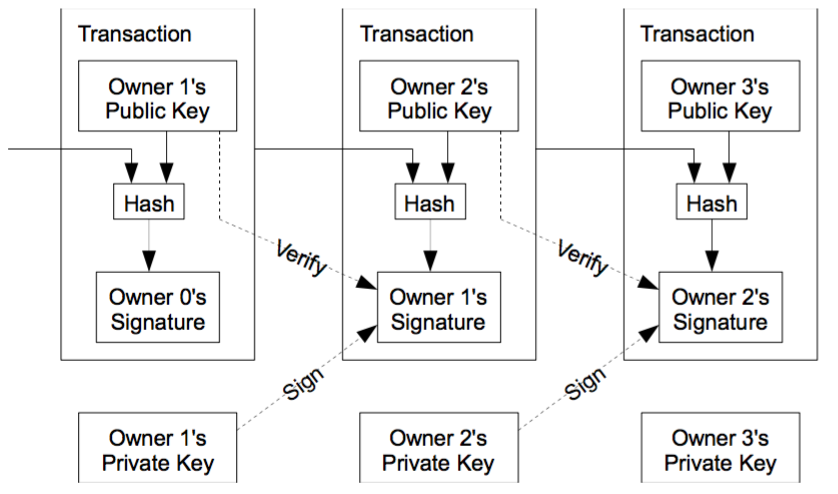
\includegraphics[scale=0.5]{figs/transactions}
\caption{Signing mechanism. Original from~\protect\cite{nakamoto2008bitcoin}}
\label{fig:signature}
\end{figure}

Furthermore, transactions have to fulfil the following criteria regarding outputs they claim and create in order to be valid~\cite{decker2013information}:
\begin{itemize}
  \item An output may be claimed at most once;
  \item Outputs are created solely as a result of a transaction;
  \item The sum of the values of the claimed outputs has to be greater or equal than the sum of the values of the newly allocated outputs. Claimed outputs are Bitcoins the payer is trying to spend and allocated outputs are the amount of Bitcoins the payee accounts are going to be able to spend.
\end{itemize}

The first criteria exist so that the user cannot double spend Bitcoins. The second ensures that unspent Bitcoins need to be connected to a transaction, avoiding forging of unspent Bitcoins. The third guarantees that Bitcoins can only be transferred and not created.

In order for payees to know that previous owners did not sign any earlier transactions, transactions are broadcasted through the Bitcoin network~\cite{nakamoto2008bitcoin}. This feature is required to ensure the payee that the payer did not already spend the Bitcoins he is using to pay him. However, this feature introduces inconsistencies in the system because transactions reach different nodes at different times:
\begin{itemize}
    \item A node could receive a transaction that transfers Bitcoins from owner \textit{B} to owner \textit{C} but that node has yet to receive the transaction that transferred the Bitcoins from owner \textit{A} to owner \textit{B}. Which might result in either the transaction not being accepted or a longer time to be accepted.
    \item A node could also receive two transactions from the same owner \textit{A} where he tries to transfer the same Bitcoins to two different payees \textit{B} and \textit{C}. This is a case of double-spending.
\end{itemize}

As there is no guarantee that different nodes receive conflicting transactions in the same order, those nodes will disagree on those transactions and any transactions built on top of them by claiming their outputs~\cite{decker2013information}. This would have been a problem because they would not agree upon a common record. For instance, if a user sent his transaction to node \textit{A}, \textit{A} would accept it because in its record the user had those Bitcoins to spend. But if the user had sent his transaction to node \textit{B},  \textit{B} might not have accepted it because in its record the user had never been the owner of the Bitcoins he is trying to transfer. We will see how this problem is solved by Bitcoin in the next section.

\subsection{Blocks}
\label{sec:blocks}

Since different nodes can commit transactions in a different order, as seen previously, they need to have a way to reach a consensus on the set of transactions that are considered valid. The role of the blocks is precisely to allow nodes to agree upon a set of transactions.

Each block is composed of a set of transactions, a nonce, a pointer to its parent block and other fields not relevant for this explanation. Each block is also associated with a block header that summarizes the information in that block.

In order for a block to be accepted by other nodes it has to present a~\acrlong{pow} (\acrshort{pow}). \acrshort{pow} consists in finding a byte string, called nonce, that hashed with the block header results in a hash with a given number of zeros at the beginning. That number of zeros at the beginning is also called \textit{target}~\cite{decker2013information}. As cryptographic hash functions are only one-way, discovering such nonce can only be done by trial and error. Furthermore, the difficulty of the \textit{target} is also adjusted. The Bitcoin network measures how much time it took to create the last 2016 blocks in a blockchain. If it took significantly more than 2 weeks, the \acrshort{pow} difficulty is reduced, meaning that there will be fewer zeros at the beginning of the next \textit{target}. If it took significantly less than 2 weeks, the difficulty is increased. Due to the very low probability of successful generation, it's unpredictable which miner nodes in the network will be able to generate the next block.

The \acrshort{pow} is necessary because it adds a real-world cost to produce a block. So with the requirement of a block having to present a \acrshort{pow}, it becomes infeasible for people to modify the history of the system and present it as the truth to anybody else as we will see in Section~\ref{sec:51attack}.

To incentivise miners for having spent resources on finding the \acrshort{pow}, each time a new block is created a new Bitcoin is generated~\cite{decker2013information}. The reward transaction is only valid if it appears in a block. This transaction is also the only transaction that is the exception to the third criteria seen in the Section~\ref{sec:transactions} which states that the sum of the inputs has to be greater or equal to the sum of the outputs~\cite{decker2013information}.

Today as the number of transactions increases on a daily basis and given the limited space each block has for transactions (1MB), miners also profit through fees imposed on transactions. Most miners choose which transactions to include in their blocks based on how profitable they expect those transactions to be. If there are two transactions of equal byte size but only one of them fits in a block, then the miner will choose whichever transaction has the higher transaction fee.

When a node finds a new block, it broadcasts it to the other nodes. Upon receiving a new block, two things can happen:
\begin{itemize}
\item The node will rollback all tentatively committed transactions since the last block reception and then commit the ones on the new block~\cite{decker2013information}. Tentatively committed transactions are transactions that were valid and would have been committed if the node had been able to generate a new block.
\item The node has already mined or received a new block and it will ignore the newly received block. The implications of this are further discussed in Section~\ref{sec:blockchain}.
\end{itemize}
%At this point, all nodes have agreed on the validity of all transactions on the block \cite{decker2013information} and the network has been synced.

Regarding the tentatively committed transactions that were rolled back, if they were present in the new block they do not have to be re-applied. For those that were not, they will be re-applied only if they are valid. Invalid transactions are transactions that conflict with one or more transactions that were present in the new block. If a transaction is flagged as invalid it will be discarded~\cite{decker2013information}. The node that created the invalid transaction will eventually receive the block with the valid transaction and it will have to rollback the invalid transaction.

Because of this feature, the creator of the block imposes over the network which transactions are going to be committed and what is the order that they are committed~\cite{decker2013information}.

In the next section, we will see how blocks are linked together to create a distributed record of what happened.

\subsection{Blockchain}
\label{sec:blockchain}
As we have seen, blocks are used by nodes to agree on the order of recent transactions. Furthermore once a block is generated it is also linked with the block that preceded it. This creates a chronological order over all blocks and therefore transactions as seen in Fig.~\ref{fig:blocks} this chain of blocks is called \textit{blockchain}~\cite{decker2013information}. The first block in the chain is called the genesis block.

\begin{figure}[h]
\centering
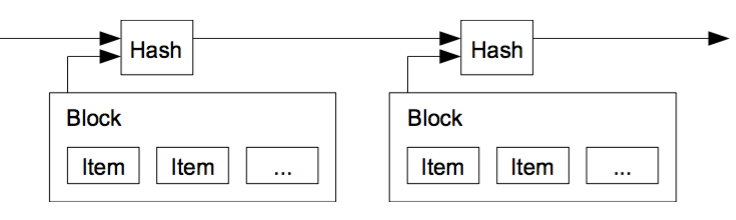
\includegraphics[scale=0.65]{figs/orderBlocks}
\caption{Blockchain representation. Original from~\protect\cite{nakamoto2008bitcoin}}
\label{fig:blocks}
\end{figure}

The blockchain is defined as the longest path from any block to the genesis block. This definition makes the blockchain resemble a tree where the root is the genesis block and the leaves are the new blocks. The height of a block is the distance of that block to the genesis block. The block that is the furthest away from the genesis block is called the blockchain head~\cite{decker2013information}.

As only new blocks are rewarded with new Bitcoins, miners try to build on top of the blockchain head~\cite{decker2013information}. This is because if they were to build on top of previously found blocks it would require them to first reach the same height as the blockchain head and then find the new block~\cite{nakamoto2008bitcoin}. Which is very hard to do because they would have to re-find all the previous \acrshort{pow} and a new \acrshort{pow} while competing against the rest of computational power present in the network. For a miner to have success at doing this he would have to control at least 51\% of the computational power in the network, we will discuss this in section~\ref{sec:51attack}.

As seen in Section~\ref{sec:blocks}, a node can accept a new block or ignore it. Because of this, there might be multiple blocks at the same height at any point in time. This is called a \textit{blockchain fork}. Hence, when this happens the network does not agree on which block is the blockchain head. This leads to inconsistency of the system because both block \textit{b} and block \textit{b'} are guaranteed to disagree on some transaction. This will go on until one of the branches overtakes the other~\cite{decker2013information}.

When a node has as blockchain head the block \textit{b} and it receives a new block \textit{b'} where the height of \textit{b' \textgreater b} two things can happen depending on which branch \textit{b} is in:
\begin{itemize}
\item If \textit{b} is in the same branch as \textit{b'} then the node only has to apply all transactions in the intermediate blocks incrementally, if any, and then apply the transactions in \textit{b'},
\item If \textit{b} is on another branch then the node is required to change branches. This implies that the node has to revert all transactions it has been committing until it reaches a common block ancestor. Then, it has to request all intermediate blocks apply the transactions in those blocks and finally apply the transactions on \textit{b'}~\cite{decker2013information}.
\end{itemize}

The fork may be prolonged throughout multiple block heights \textit{h, h+1, h+2...} where subsets of the network work on the different branches and try to find new blocks at the same time. Eventually one of the branches will surpass the others, leading to the adoption of this branch by all the nodes and sequentially the end of the blockchain fork~\cite{decker2013information}. The discarded blocks are called \textit{orphan blocks}.

As a consequence of blockchain forks, a transaction in Bitcoin is never committed permanently. Because at any point in time it could appear a branch that was not known by the nodes we were interacting with which might influence the state of our transactions. If this new branch is taller than the one where our transactions were confirmed then our transactions will be rolled back else they will not be affected.


\subsection{Network}
\label{sec:network}
Bitcoin is supported by a network of peer-to-peer nodes that mine new Bitcoins, create and disseminate transactions and keep a record of what transactions happened. This network has two components that should be looked into to understand some of the vulnerabilities that we will study in the next section. Those two components are:

\begin{enumerate}
	\item Network overlay - how the Bitcoin peer-to-peer network is built;
	\item Information propagation - how does the Bitcoin protocol forward information.
\end{enumerate}

\subsubsection*{Network overlay}
\label{sec:p2pnetwork}

When a node wants to join the network there are five ways for it to connect with peers~\cite{bitcoinwiki}:

\begin{enumerate}
	\item Address database - this file contains other nodes that the node already knew about, the node will try to re-connect with those nodes. If it is the first time the node connects to the network this method doesn't work;
	\item User-specified - in this method the user can specify nodes to connect to on the command line;
	\item DNS seeding - this option is only used if the Address database file is empty and the user did not specify any nodes. The nodes issue DNS requests to a list of 6 DNS servers that are hardcoded in order to discover IP addresses of other peers, each DNS server can return up to 256 IP addresses;
	\item Hard-coded nodes - If DNS seeding fails, the node contains a list of 1525 hard-coded IP addresses that represent bitcoin nodes that IT contacts to get addresses of other peers and then finishes the connection with them to avoid overloading those nodes;
	\item From other nodes - Nodes exchange IP addresses with other nodes via the \textit{getaddr} and \textit{addr} messages which we will discuss later.
\end{enumerate}

By default a node connects to a minimum of 8 outbound peers (connections initiated by this node) and allows up to 125 inbound peers (connections initiated by other nodes). This limitations exist to prevent nodes from being isolated and to prevent nodes from becoming essential to the system. For instance, if a node was responsible for connecting all the nodes of Europe with all ones from Asia if that node failed the system would collapse.

%TODO this needs to be reworked from here
\todo{This part has to be reworked} Once connected to the network nodes exchange among them the addresses of other nodes, using the \textit{getaddr} and \textit{addr} messages, to maintain the network overlay up to date.
Usually, an \textit{addr} message is sent in response to a \textit{getaddr}. However, the \textit{addr} message may also arrive unsolicited, because nodes advertise addresses gratuitously when they \cite{bitcoinwiki}:
\begin{itemize}
\item Relay addresses - once a node adds to its list of neighbours a newly received IP addresses it may relay it to other nodes if certain conditions are met;
\item Advertise their own address - every 24 hours, the node advertises its own address to all connected nodes;
\item Establish a connection;
\end{itemize}
In order to maintain a connection with a peer, nodes by default will send a message to peers before 30 minutes of inactivity. If 90 minutes pass without a message being received by a peer, the node will assume that connection has closed \cite{bitcoincorewiki}.

There are also organizations called \textit{mining pools}, composed by multiple nodes that work together to find the \textit{PoW} more efficiently. In mining pools each node test different nonces to find the \textit{PoW} which is faster than a single node testing all the possible nonces. \textit{Mining pools} are composed by multiple nodes and gateways that connect the pool to the Bitcoin network. Once they find a \textit{PoW} and generate a block the reward is then split among the members of the pool that worked on that \textit{PoW} proportionately to the contribution that each member made.
%TODO until here
\subsubsection*{Information propagation}
\label{sec:dataexchange}
In order to exchange messages a Bitcoin node has to each of its neighbours, a message queue with messages that will be sent once a timer associated with each queue ends.

\paragraph*{Transactions}
The usual way transactions are relayed to other nodes works as follows. Node \textit{A} creates a new transaction, \textit{A} will add the advertisement for that transaction to the message queue of all his neighbours. If \textit{A} learns that one of it's neighbours already has that transaction, it will remove the advertisement for that transaction from the queue of that neighbour. Once a neighbour \textit{B} receives the advertisement it will check if it already has that transaction and if it does not it will sent to \textit{A} a \textit{GetData} requesting the new data. Node \textit{A} will then send the requested data individually meaning that if it receives a request for ten transactions it will send ten separate messages. Once \textit{B} receives the new transaction it will verify if it is valid and if it is it will also relay it through his neighbours.

Transactions can also be sent unsolicited.

\paragraph*{Blocks}
Until Bitcoin version 0.13.0 (23-08-2016) the usual way to relay blocks was similar to the way transactions are relayed. However with the addition of new message compact blocks this changed. Although blocks can still be relayed through advertisements the main method for relaying a block between uptodate nodes is through compact blocks. The difference between the two methods of relaying is that, through advertisements once a node \textit{A} sends a \textit{Block} message replying to a \textit{GetData} message, the message \textit{Block} has all the contents of the block which gives to the receiving node the ability of fully validating the block. In the case of a \textit{CMPCTBLOCK} message, \textit{A} will only send crucial information to \textit{B} so that it is able to reconstruct the block, this means that some information like transaction are summarise and only sent their id's. This process of relaying blocks is an improvement over the previous method because it reduces the amount of bandwidth consumed when sending blocks. If for instance a node does not have all the transactions necessary to rebuild a block it will send a \textit{GetBlockTX} message to the node that sent him the compact block. Once a node receives a \textit{GetBlockTX} it will respond with a  \textit{BlockTX} message containing all the missing transactions.

This way there are in total tree ways a block can be relayed as we can see in Fig. %TODO add figure
%There are tree ways a node can relay transactions, that either he created or received:

%begin{itemize}
%\item \textbf{Advertisemnts} - the node will add advertisements to the message queue of each neighbour, only if he thinks that the neighbour still does not has that transaction;
%\item \textbf{Direct} - the node will simply send the transaction,  if he thinks that the neighbour still does not has the transaction;
%\item \textbf{GetBlockTX} - the node will send an array of transactions as a response to a GetBlockTX.
%end{itemize}


%When new transactions (\textit{txs}) or blocks (\textit{blocks}) are created, the node \textit{A} that generated them will broadcast an \textit{inv} message. This message contains information regarding \textit{txs} and \textit{blocks} that \textit{A} knows about.

%Once a node \textit{B} receives an \textit{inv} message that contains a \textit{tx} or \textit{block} that he does not have, it will reply to \textit{A} with a \textit{GetData} requesting the new data. Upon receiving the \textit{GetData} message, node \textit{A} will then send the requested data.

%Finally, once node \textit{B} receives the new data it will verify it. If the new data is valid, it will also announce it to its neighbours with a \textit{inv} message.

%\textit{Txs} and \textit{blocks} are not broadcast directly to the network because of the size of \textit{blocks} and the high frequency of both of them. By sending \textit{inv} messages Bitcoin also avoids nodes from receiving multiple times the new \textit{tx}/ \textit{block}.

There are also messages that allow, nodes that were disconnected from the network, to quickly get the data that they have missed. These messages are especially useful because it speeds up the process of gathering data for the creation of blocks. They are also useful when nodes do not have the parent block of a block they just received, they can use these messages to ask their neighbours for the missing block \cite{bitcoincorewiki}.

\subsection{Summary}
%TODO rework img
In conclusion, Bitcoin is made up of multiple modules as seen in  Fig.~\ref{fig:bitcoinoverview}. We will briefly describe them~\cite{bitcoinwiki}.

\textit{Txs} and \textit{Blocks} represent transactions and blocks respectively.

\textit{Mempool} is the place where the node stores the transactions that are going to be included in next blocks. The \textit{Validation Engine} is in charge of validating the transactions/blocks that are received. The \textit{Miner} is the module responsible for mining blocks. Finally, the \textit{Storage Engine} is the module that manages all the databases where a node stores all the relevant data like \textit{Blocks}, \textit{Blocks Headers} and \textit{Coins}.

The \textit{Wallet} is the module where the Bitcoins of the user are stored and the \textit{RPC} module is used so that applications can interact with Bitcoin, hence providing an API to the outside.

The modules that we are more interested in are the \textit{Peer Discovery} and the \textit{Connection Manager} because of their connection to the network aspect of Bitcoin. The \textit{Peer Discovery} is responsible for building the Network and maintaining it. The \textit{Connection Manager} is accountable for managing the way data and control messages are broadcasted.

\begin{figure}[h]
\centering
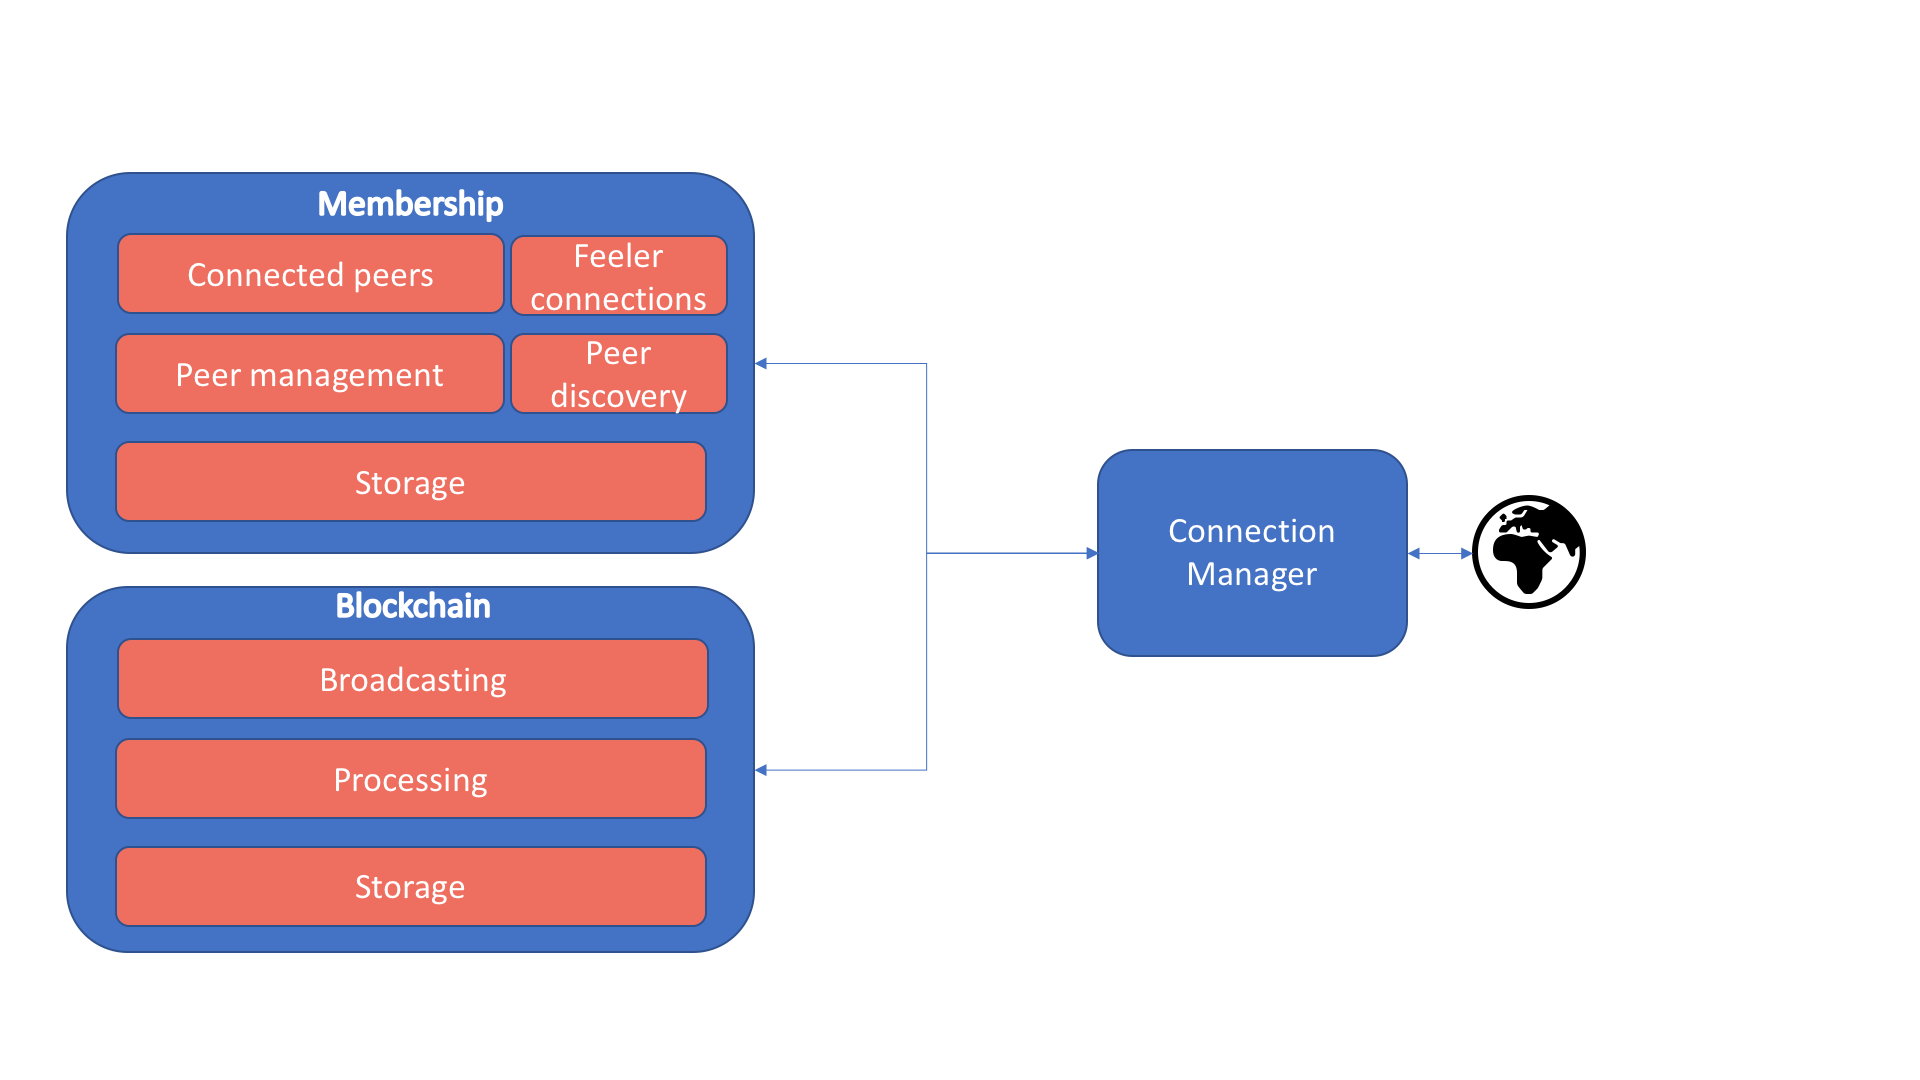
\includegraphics[scale=0.4]{figs/My-Bitcoin-Core-architecture}
\caption{Bitcoin architecture (Source Eric Lombrozo)}
\label{fig:bitcoinoverview}
\end{figure}

Next, we will take a look at some of the vulnerabilities of Bitcoin and compare it with other cryptocurrencies to understand which modules have to be modified in order to fix those problems.


%O sistema Bitcoin~\cite{nakamoto2008bitcoin} foi criado em 2008 com o objetivo de disponibilizar um meio seguro e anónimo onde duas entidades possam realizar transações entre si sem terem de confiar em terceiros. Para este propósito o sistema possuí uma criptomoeda que pode ser trocada entre várias entidades envolvidas numa transação. Todas as transacções são agrupadas em blocos e registadas num livro-razão, mantido de forma descentralizada. Para além de manter um registo das transacções, o livro-razão permite também seriar todas as transacções e, desta forma, evitar que um utilizador use as mesmas moedas em mais que uma transacção (fenómeno designado na literatura anglo-saxónica por \emph{double spending}).
%O livro-razão da Bitcoin  é construído ligando cada bloco ao seu predecessor formando uma corrente infinita de blocos conhecida como a \textit{blockchain}.

%O protocolo para manter o livro-razão na Bitcoin é relativamente complexo, e inclui várias funcionalidades que se complementam. Em primeiro lugar, a Bitcoin corre algoritmos de filiação, que tentam assegurar que cada nó mantêm ligações com outros nós do sistema escolhidos de forma aleatória. Estas relações de vizinhança criam uma rede sobreposta que é usada para disseminar informação na rede, nomeadamente: informação sobre as transacções submetidas pelos clientes e informação sobre os novos blocos da cadeia.

%Como referimos anteriormente, os novos blocos da cadeia são gerados de forma concorrente por nós designados por mineiros. Cada mineiro recolhe um conjunto de transacções que conhece, que agrupa num bloco. Para o bloco ser válido, para além de todas as transações que inclui necessitarem de ser válidas, tem de conter a resposta a um puzzle criptográfico computacionalmente exigente que depende, entre outros, do bloco anterior e das transacções incluídas no novo bloco. Isto tem duas vantagens. Em primeiro lugar, desencoraja a criação de blocos incluindo transacções inválidas, uma vez que a única forma de um mineiro ser compensado pela energia gasta na resolução do puzzle é através da aceitação do seu bloco na cadeia. Para além disso, a dificuldade do puzzle reduz a probabilidade de dois mineiros gerarem blocos simultaneamente, o que limita a ocorrência de bifurcações na cadeia. Note-se que, uma vez que as transacções demoram a ser propagadas pela rede, é provável que quando dois mineiros tentam concorrentemente criar um novo bloco, não usem exactamente o mesmo conjunto de transacções e, portanto, não tenham de resolver o mesmo puzzle. Assim que um novo bloco é gerado, este é propagado na rede. Para evitar a propagação de blocos mal formados, cada nó valida o bloco antes de o propagar. Para verificar a correcção de um bloco, um nó deve possuir a seguinte informação: registo dos blocos anteriores (uma vez que cada bloco, contém uma referência para o bloco anterior) e ter informação sobre as transacções que estão incluídas nesse bloco, de forma a validar a sua autenticidade. Se um nó não possuir esta informação, tem que a solicitar primeiro, esperar que esta esteja disponível localmente, e só depois pode dar continuidade à propagação dos blocos.

%Se um mineiro recebe o n-ésimo da cadeia enquanto ele próprio o está a tentar gerar, o processo de criar um novo bloco é abortado. Este mecanismo faz com que a probabilidade de se gerarem duas versões distintas, criando uma bifurcação, seja muito pequena. Nos casos em que uma bifurcação acontece, o desempate é feito com base no comprimento de cada ramo. Quando um nó se apercebe que está a trabalhar sobre uma bifurcação que não é a mais longa, descarta essa bifurcação e junta-se ao ramo (que considera ser o) principal.

%Os algoritmos usados na Bitcoin para propagar blocos e transações têm evoluído com o tempo, e incluem um conjunto de mecanismos que pretendem evitar o desperdício de largura de banda na rede.
%Descrevemos de seguida sucintamente o protocolo.
%Como referido anteriormente, as transações são disseminadas através de mensagens de anúncio \textsl{Inv} que contêm um conjunto de transações conhecidas pelo emissor.
%Ao receber uma mensagem de \textsl{Inv}, o receptor determina quais as transações que desconhece e pede-as ao emissor, enviando-lhe uma mensagem de \textsl{GetData} que, por sua vez, responde com uma mensagem \textsl{TX} por cada transação pedida.
%Os blocos são disseminados através de duas estratégias distintas.
%A primeira estratégia, e também a mais antiga, consiste em anunciar blocos através de mensagens \textsl{Headers}.
%Caso o bloco seja desconhecido, ou algumas das transações que o compõem, esse bloco é pedido através da  mensagem \textsl{GetData}, sendo o bloco completo enviado através de uma mensagem \textsl{Block}
%que contem toda a informação necessária para validar o bloco.
%Caso o nó não conheça o predecessor do bloco a ser anunciado pode requisitar o cabeçalho deste com uma mensagem \textsl{GetHeaders}.
%A segunda estratégia consiste em enviar somente um sumário do bloco, através de uma mensagem de \textsl{CmpctBlock} (bloco compacto).
%Caso o bloco ainda não seja conhecido, o nó valida o bloco, pedindo ao emissor as transações desconhecidas, se alguma, através de uma mensagem \textsl{GetBlockTX}.
%A primeira estratégia evita a troca adicional de mensagens mas, no entanto, resulta em mais redundância pois como as transações são disseminadas concorrentemente com os blocos é provável que a maior parte das transações de um bloco já sejam conhecidas por um nó.


%Adicionalmente, os nós mantêm, para cada vizinho, uma fila de saída que contêm as mensagens a ser enviadas no futuro.
%Quando uma nova mensagem de \textsl{TX} é recebida, esta é colocada na fila de todos os vizinhos.
%À medida que se recebem anúncios e blocos de vizinhos estas filas são atualizadas para evitar enviar de volta transações que os vizinhos já conhecem.
%Periodicamente, estas filas são percorridas e é enviado aos respetivos nós um \textsl{Inv} que contêm as transações conhecidas localmente, permitindo que o destinatário peça as mensagens desconhecidas conforme indicado acima.

%Embora já existam algumas preocupações em reduzir o número total de mensagens trocadas, bem como a quantidade de informação, este mecanismo ainda possuí várias ineficiências que discutimos na secção seguinte.



\section{Bitcoin and Blockchain vulnerabilities}
\label{sec:vulnerabilities}
In this section, our objective is to look at known vulnerabilities of Bitcoin, as well as, look into the solutions proposed to those vulnerabilities. We will also compare Bitcoin with other cryptocurrencies to see where Bitcoin stands in comparison to the state of the art.

This section is divided into four sections, one for each of the main vulnerabilities we have identified.

\subsection{Information Eclipsing}
\label{sec:ieclipsing}
This vulnerability was found in \textit{Information Propagation in the Bitcoin Network} \cite{decker2013information} and it happens because of following behavior. Lets consider that the whole network recognizes a block \textit{b} at height $H_b$ as the blockchain head. Then at two different locations of the network two new blocks are discovered. These blocks are guaranteed to be different as seen in Section \ref{sec:blocks}, lets call each one \textit{b'} and \textit{b''}.

Now both blocks are going to be broadcast through the network because both are at height $H_{b+1}$. Hence, when a node receives either \textit{b'} or \textit{b''} it will consider it as the new blockchain head and will broadcast it to its neighbours. The problem is, when a node that already received \textit{b'} receives \textit{b''} or vice-versa that node will not broadcast \textit{b''} through the network as it did with \textit{b'}, because it already moved to a new blockchain head at the same height. As a consequence, only nodes that received both \textit{b'} and \textit{b''} know about the existence of a fork. This diminishes the effective computational power in the network because the network will be working on different blockchain heads. Hence, empowering some of the attacks in the following sections.

The authors of the paper discovered that it takes 6.5 seconds for the block to reach 50\% of nodes, 40 seconds for it to reach 95\% of nodes and that the mean delay for a block to be reach a node in the network is 12.6 seconds. Since Bitcoin has a block creation time of 10 minutes the authors concluded that the effective computational power in the Bitcoin network is only 98.20\%. This happens because once a block is found it takes in mean 12.6 seconds to reach a node, so in mean during those 12.6 seconds the rest of the network is wasting resources, resources that do not contribute to extend and strengthen the blockchain.

If we wanted to use Bitcoin for faster transactions, then the block time would have to go down. But if we maintain the 12.6 propagation delay and decrease the block time the effective computational power would also decrease even more as showcased in \cite{ethereumblog}. The intuition is that with a lower block time the probability of stale blocks\footnote{Blocks that were candidates to being the next blockchain head but were not chosen.} being created increases. This will result in more forks being created and more resources more wasted resources.

Regarding solutions, the authors suggested multiple options to optimize the propagation of a block, which would lower the 12.6 seconds delay and the lower probability of stale blocks being created. One of the solutions consisted in changing the block verification process. In this solution, the verification of a block would be split into two phases an initial difficulty check and a transaction validation. Since the transaction validation is the phase which takes longer, a node would perform the initial difficulty check where it checks the validity of the \textit{PoW} and once this was done the node could broadcast the \textit{inv} messages right away while performing the transaction validations asynchronously.

Ethereum solved part of this problem through the implementation of uncle blocks. Rather than discarding stale blocks as in Bitcoin, Ethereum includes them in new blocks, hence the name uncle blocks. Uncle blocks are included in new blocks up to a certain height difference between the uncle block and the new block being generated. This happens because nodes that generated uncle blocks are rewarded with a fraction of the full reward, so the limit imposed by the height difference avoids having a group of nodes mining on lower heights.

With this solution Ethereum solved this problem because now blocks to be built also include other previously built blocks in addition to the already included parent block. This means that no computational power is lost. Because for an attacker to forge a block he would need to remake all previous blocks of the main chain and all the uncle blocks of that block, since uncle blocks also had the transaction that the attacker is trying to eliminate. This attack is further explained in the next section.

The disadvantage of this solution is the extra computational power and memory required to include the uncle blocks.

\subsection{51\% Attack}
\label{sec:51attack}
The 51\% attack was first introduced in the original Bitcoin paper \cite{nakamoto2008bitcoin}. This attack requires the attacker to control 51\% of the computational power available in the network, hence the name. Given the inefficiencies in the propagation of messages through the network seen previously the required computational power to perform the attack is actually 49.10\% \cite{decker2013information}. Once the attacker is able to obtain this computational power it will proceed to rebuild blocks erasing transactions where he was the payer. Note that this is the only thing the attacker can do because nodes would never accept a block with forged transactions. This is because valid transactions require the signature of the payer.

Although this attack is possible, it is very hard to perform because the attacker would need to rebuild not only the block where his transactions were present, but he would also need to rebuild all the blocks built on top of that block until he reached the blockchain head and overtook it, making his branch longer. As a consequence, this would result in the rest of the network considering that branch as the main branch, leading to the success of the attack. But as Satoshi Nakamoto explained in \cite{nakamoto2008bitcoin}, if the attacker does not catches up to the blockchain head early on and overtakes it the difficulty of the attack will increase. Because more blocks will be built on top of the main chain hence he will have more blocks to generate.

%It is also worth noticing that the authors in \cite{decker2013information} reached the conclusion that given some inefficiencies in the propagation of messages through the network, the effective computational power in the network is 98.20\% which means that the attack is possible if an attacker controls 49.10\% of the computational power as we say in Section \ref{sec:ieclipsing}.

This attack is possible because of the way consensus is reached in Bitcoin. Bitcoin reaches consensus by considering the main branch of the blockchain the taller branch on the blockchain tree. So if someone was able to control 51\% of the computational power he could generate a taller branch which would make the rest of the network consider that the main branch. Hence this problem cannot be solved unless we were able to control who joins the network.

Other coins affected by this problem tried to solve the problem in different ways. Ethereum for instance, started using uncle blocks as we have seen in the previous section. This solution does not solve the problem because an attacker could still gather enough computational power to remake all the uncle blocks and blocks in the main branch. But it makes it harder for the attacker to perform the attack as it described in Section \ref{sec:ieclipsing}.

Ripple is also not affected by this attack because in ripple consensus is not connected with computational power. In ripple, the consensus is achieved by a set of trusted nodes called validators. Validators are chosen based on the expectation they will not collude in a coordinated effort to falsify data relayed to the network. A disadvantage of this approach is that it removes decentralization characteristics of the cryptocurrency. In Bitcoin, everyone ``votes" when they start trying to mine on a block in Ripple power of ``voting" is removed from the users.

%TODO add ripple comment

\subsection{Partition Attack}
This attack allows an adversary Autonomous System (AS) level to isolate a set of nodes from the rest of the network using the Border Gateway Protocol (BGP) hijack.

BGP hijack consists in injecting forged information in the network on how to reach one or more IP prefixes, leading other ASes to send traffic to the wrong location.

The attack starts by the given AS diverting the traffic destined to a certain set of nodes (which we will call \textit{P}) through BGP hijack. This means that all traffic destined to \textit{P} goes to the AS instead. Then, the AS will examine the traffic being sent to \textit{P} and it will drop every message that has a Bitcoin header in the TCP payload. The rest of the traffic is considered irrelevant and reaches \textit{P}.

During the interception of traffic, there can be two types of relevant traffic: i) traffic crossing the partition from the outside to the inside; ii) traffic that appeared from inside the partition. In the first case, the AS only has to drop Bitcoin messages but in the second case, the AS has to analyse the exchanged Bitcoin messages to detect the ``leakage points", which are nodes that have connections to the outside of the partition that the AS cannot control.

To accomplish this, the attacker checks, for every packet, if the sender belongs to \textit{P}. If the sender belongs to \textit{P} the attacker will check whether the sender is advertising information from outside \textit{P}. Particularly, the attacker checks whether the packet contains an \textit{inv} message with the hash of a block mined outside of \textit{P}. If yes then the sender was a ``leakage points"  \cite{apostolaki2016hijacking}.

Once the AS finds out the ``leakage points" it will exclude them from \textit{P}, successfully isolating the nodes in \textit{P} from the rest of the network.

This attack leads to different consequences depending on the number of nodes successfully isolated. If the number is low the impact of the attack is basically a Denial of Service and the nodes within \textit{P} have zero confirmation for double spending. If the number of nodes is high it might result in revenue loss for miners and the side with higher computational power will decide which transactions are committed because they will generate blocks faster. This aspect will be discussed in more detail in Section \ref{sec:rpsummary}.

Regarding solutions for this attack in \cite{apostolaki2016hijacking} the authors suggest, increasing the diversity of the node connections while taking routing into account, monitoring the RTT because the RTT value would increase if a node was being attacked and a few others.

The success of this attack depends on the protocol used by the ASes to advertise addresses. For instance, if BGP was not used by the ASes this attack would not be possible. Still, a module that can be changed in Bitcoin to address this problem is the \textit{Peer Discovery}. Because this module should establish more resilient connections.

In Ethereum and Ripple, this attack is not possible as the connections between nodes are encrypted which would make impossible the analysis of traffic that the AS would need perform. But they sacrifice performance.

\subsection{Delay Attack}
The objective of this attack is to slow down the propagation of new blocks sent to a set of nodes without disrupting their connections \cite{apostolaki2016hijacking}.

The mentioned attack has two different ways of being performed depending on the direction the attacker is able to intercept the traffic: in the victim network \textit{V$\,\to\,$N} direction or network victim \textit{N$\,\to\,$V} direction.

If the attacker is able to intercept the connection in the \textit{V$\,\to\,$N} direction then the attack works as follows. When the victim requests a block to the network the attacker will change the block request to another block which will lead the victim waiting for a response. After almost 20 minutes, time limit where the victim requests the block to another neighbour, the attacker will modify another message sent by the victim to that neighbour, probably a transaction request since are the most common message type, to request the initial block that the victim wanted. This way the attacker avoids the victim from dropping the connection with that neighbour, which allows the attacker to perform the attack multiple times.

If the attacker is able to intercept the communication in the other direction \textit{N$\,\to\,$V}. In this direction, once the victim requests a block to a neighbour the attacker will intercept and tamper with the response (the block itself) corrupting it, which will lead to it being discarded by the victim. But the victim will not request the corrupted block again. Then, after 20 minutes the victim will drop that connection because the block never arrived and will request the block to another neighbour. Hence, the attack performed this way can only be done once.

The impact of this attack depends on the node that is being attacked if it's a simple node then this attack will be a Denial of Service and that node will not have guarantees for double spending if that attack is towards a gateway of a pool it could be used to engineer block races.

This attack is successful because Bitcoin connections are not tamper proof and Bitcoin does not requests the block again when presented with a corrupted block, this is a problem related to the \textit{Connection Manager} module.

A solution for this attack is monitoring the RTT, as the RTT increases considerably when the node is being attacked. Other solution proposed in \cite{apostolaki2016hijacking} is encrypting Bitcoin communications which would not avoid the packets from being dropped by an attacker but it would prevent them from eavesdroppping and tampering with connections. The disadvantage with this approach is that it would require additional computations making the system slower.

Ethereum and Ripple are not affected by this attack as all the connections are encrypted but the attacker can still drop packets. But they sacrifice performance.


\subsection{Summary}
We have analyzed several attacks that can be performed against Bitcoin. Table \ref{fig:tabel1} summarizes these attacks for Bitcoin but also for other popular cryptocurrencies. For some attacks, we were unable to assess if the attack was really possible due to some undocumented parts of the cryptocurrencies. These are noted in the table as "Might be affected by the attack".

We can see in Table \ref{fig:tabel1} that all the cryptocurrencies related with Bitcoin like \textit{Bitcoin Cash} and \textit{Bitcoin Gold} suffer from the same vulnerabilities as Bitcoin. Whereas all cryptocurrencies not relatable with Bitcoin have for the majority of the attacks found a solution for them or at least a minor fix. This happens because unlike those cryptocurrencies Bitcoin does not have an organization that can make decisions on its own regarding the direction of the cryptocurrencies, as seen recently by the Segweit agreement. So when decisions have to made it takes a lot of time for the community to reach a consensus and sometimes these decisions even lead to forks of the cryptocurrencies which decreases the value of the cryptocurrencies.

It is also worth noticing that although cryptocurrencies not relatable with Bitcoin have solutions for the vulnerabilities described they had to sacrifice other characteristics. Ethereum for instance sacrifices performance because all its connections are encrypted and uncle blocks are used. Ripple has pour privacy features and also sacrifices performance because its connections are also encrypted.

\begin{table}[]
\centering
\begin{tabular}{l|c|c|c|c|c|c|}
\cline{2-7}
 & \begin{tabular}[c]{@{}l@{}}Bitcoin\\ bitcoin.org\end{tabular} & \begin{tabular}[c]{@{}l@{}}Ethereum\\ ethereum.org\end{tabular} & \begin{tabular}[c]{@{}l@{}}Bitcoin Cash\\ bitcoincash.org\end{tabular} & \begin{tabular}[c]{@{}l@{}}Ripple\\ ripple.com\end{tabular} & \begin{tabular}[c]{@{}l@{}}Dash\\ dash.org\end{tabular} & \begin{tabular}[c]{@{}l@{}}Bitcoin Gold\\ bitcoingold.org\end{tabular} \\ \hline
\multicolumn{1}{|l|}{\begin{tabular}[c]{@{}l@{}}51\% Attack\\ \\ \end{tabular}} &  &  &  & $\checkmark$ &  &  \\ \hline
\multicolumn{1}{|l|}{\begin{tabular}[c]{@{}l@{}}Information\\ Eclipsing\end{tabular}} &  & $\checkmark$ &  & $\checkmark$ & $\bigcirc$ &  \\ \hline
\multicolumn{1}{|l|}{\begin{tabular}[c]{@{}l@{}}Partition\\ Attack\end{tabular}} &  & $\checkmark$ &  & $\checkmark$ & $\checkmark$ &  \\ \hline
\multicolumn{1}{|l|}{\begin{tabular}[c]{@{}l@{}}Delay \\ Attack\end{tabular}} &  & $\checkmark$ &  & $\checkmark$ & $\bigcirc$ &  \\ \hline
\end{tabular}
\caption{Cryptocurrencies and their respective problems. \\ $\checkmark$ - Not affected by the attack \\ $\bigcirc$ - Might be affected by the attack}
\label{fig:tabel1}
\end{table}



\section{Related Problems}
\label{sec:rproblems}
In this section we will take a look at some problems related with network membership and node behaviour. These problems have been the focus of many studies because they are important for a good and sustainable peer-to-peer network.

Bitcoin is supported by a peer-to-peer network where is expected that all nodes have a random sample of neighbours and disseminate information as soon as they receive it. But as we have seen in the previous sections this does not always happen with attacks being performed at the network level like the partition attack. Furthermore, as we will see in Section \ref{sec:rpsummary}, even some nodes inside the network do not behave properly and try to take advantage of high number of connections or selfish behaviour. However, all these problems are not new in the distributed systems field and have been the aim of a lot of research. Hence, is in our interest to look into how these problems affected other peer-to-peer technologies and study the solutions proposed to them.

We will start by looking into secure overlays in Section \ref{sec:secureoverlays}, where we will explain what secure overlays are, present some secure overlays vulnerabilities and present some approaches to building secure overlays.

In Section \ref{sec:nodesbehaviour}, will take a look at the different possible behaviours a node can have in the network, as well as, look into approaches that punish undesirable behaviours.

Finally, in Section \ref{sec:rpsummary}, we will discuss how these problems affect Bitcoin.

\subsection{Secure Overlays}
\label{sec:secureoverlays}
%Explicar secure overlays
An overlay is a network built on top of another network where peers are connected through virtual or logical links. For instance in Bitcoin, the overlay of a node is the connections that node keeps with other peers that are its neighbours.

In large systems like Bitcoin or BitTorrent is infeasible for a peer to know the overlay of the whole network, not only because of the size these networks achieve but also because peers are constantly joining and leaving. So to solve this problem peers keep only a partial list of the peers "closest" to them. Each peer is also responsible for updating and expanding his own list. To build these partial lists peers use peer sampling systems (PSS), these systems are a scalable and robust approach to building these lists. They provide every peer with a random sample of
peers to exchange information with \cite{jelasity2004peer}.

An important issue of modern PSS is their potential exploitation by malicious peers. Many of the technologies of peer sampling did not take into account attacks like the hub attack. The goal of this attack is to subvert the network in order to achieve a leading structural position hence becoming a hub. This is problematic because it can evolve in the complete defeat of the system, if the malicious nodes simply disappear after having gained such leading position.

Attacks to the PSS like the hub attack led to the creation of secure peer sampling (SPS) services. SPS use heuristics based on social network analysis to allow the system to detect and react to the structural changes in the network in a timely manner. Hence, nodes which have gained a central role in the network are identified and banned.

%Mosquito
But even attacks to SPS have been found \cite{jesi2009secure}. The objective of these attacks is to put discredit on a subset of nodes in order to disconnect or isolate them. This is achieved by a set of malicious nodes broadcasting bogus messages to discredit the victims, which will eventually lead the SPS to react by suspecting and banning those nodes, which are non-malicious. This attack is called the \textbf{Mosquito attack}.

%Superodes
Another problem that some peer-to-peer overlays like Bitcoin might have is \textbf{Supernodes}. Despite \textbf{Supernodes}  not being desirable in Bitcoin in some peer-to-peer architectures like Skype they are actually desirable and contribute to the performance of the system. Supernodes are nodes that have a number of connections higher than the average number of connections. This is a problem because these nodes start having an important role in the network and if for instance one of these nodes leaves the network the system might crash.

We will now take a look at some overlays technologies.

\paragraph*{\textbf{Secure Peer Sampling Service: The Mosquito Attack} \cite{jesi2009secure}} This system was designed to extend the SPS functionality protecting it against the mosquito attack. In this system, the attacker is considered to be a group of peers. This system introduces the concept of a knowledge base, this knowledge base is used by a peer to possibly recover its partial view in case of corruption and to detect with a good accuracy malicious peer. Peers build their knowledge base by making a stochastic proportion of their gossip exchanges as "explorative". The intuition behind this system is that since the network should be random, detecting a peer showing a popularity value too distant from the average means that it could represent a network hub. So each peer will record in its knowledge base the number of times that the address of each peer was shared with them, this value is called \textit{hits}. Once a peer identifies another peer with a high number of \textit{hits} it marks it as malicious. To protect against false negatives induced by attacks like the mosquito attack, each well-behaved peer will choose one malicious peer from their list of malicious peers and will make an explorative PS. If the results received contain more than 25\% of the already known malicious peers the suspicion is confirmed. Otherwise, the peer is removed from the list of malicious peers.

\paragraph*{\textbf{Brahms} \cite{bortnikov2009brahms}} This system was designed to provide a random sample of nodes in a large dynamic system subject to Byzantine attacks that poison the views of correct nodes. Brahms is a membership service that stores a sublinear number of ids at each node and provides each node with independent random node samples that converge to uniform ones over time. This is achieved by Brahms because in its sampler every node has the same probability of being sampled and the gossip algorithm uses two means for propagation: (1) push – sending the node’s id to some other node, and (2) pull – retrieving the view from another node. Pushes are needed to reinforce knowledge about nodes that are under-represented and pulls are needed to spread existing knowledge within the network. Brahms protects itself against poisoning attacks by limiting the number of pushes received by nodes.

\paragraph*{\textbf{Identifying Malicious Peers Before It's Too Late: A Decentralized Secure Peer Sampling Service} \cite{jesi2007identifying}} This system was built to cope with malicious nodes executing “hub attacks”. This system uses a set of multiple overlays, this means that each node belongs to different overlays, and the neighbourhood at every instance will be distinct with very high probability because the overlays have independently random-like topologies. In this system, the concept of extra caches is introduced as being the set of caches belonging to each peer; every cache in the set is a random snapshot of a distinct PSS overlay. Essentially, the multiple caches are useful in order to perceive how malicious nodes are spreading the infection from distinct directions over distinct overlays. Due to the spreading infection, is expected that common node ID patterns will emerge in all (or in the majority) of the caches. Then based on this patterns, each peer can build a set of statistics in order to guess or detect who are the malicious nodes. If a node is detected as malicious the node will decline gossip from that node.

\paragraph*{\textbf{MACHETE} \cite{raposo2016machete}} This system was designed to establish an overlay network and scatter data over the available paths, thus reducing the effectiveness of snooping attacks. Thus, it protects against passive attackers that eavesdrop on communications at certain physical locations. This system sends data through multiple paths using multiple interfaces that the computer has available, hence protecting against snooping attacks. In contrast to the other systems presented previously in MACHETE, the client is provided with the full overlay of the system when he wants to send a message. Then the client will choose the best path according to its RTT value. This system is interesting to us because of its feature of sending data through multiple paths, something that if applied correctly to Bitcoin could protect against certain attacks as we will see in Section \ref{sec:arc}.
This tool is not like the other PSS presented because it provides every client with a full view of the network instead of a partial view.

\subsection{Node's Behaviour}
\label{sec:nodesbehaviour}
In general, nodes can adopt different behaviours with respect to the specification of the protocol they are supposed to follow, namely, there are three types of nodes \textit{altruistic nodes},  \textit{byzantine nodes} and \textit{rational nodes}. \textit{Altruistic nodes} are nodes that follow the specified algorithm and are willing to disseminate information. \textit{Byzantine nodes} are nodes that generate arbitrary data, and can behave in an arbitrary way, including pretending to be a correct one. \textit{Rational nodes} are nodes that instead of strictly following the algorithm do what is best for them. For example, in the case of file sharing, a \textit{rational node} is a node that only provides small rates of upload while having a high rate of download. These nodes are harmful to the system because they do not contribute to it, for instance, if all nodes were to follow the same logic there would not be enough seeders to support the network and the system would collapse \cite{li2006bar, cohen2003incentives}.

It is important to look at these behaviours and the approaches to punish them because although it would be desirable that in the Bitcoin network all nodes behaved well that is not the case. This will be further discussed in Section \ref{sec:rpsummary}.

Next, we discuss how some approaches deal with some of these possible behaviours.

\paragraph*{\textbf{BitTorrent} \cite{cohen2003incentives}}
The approach described in this paper was conceived to cope with free riders in a file sharing network. A free rider in this systems is a peer that is trying to have the highest possible download rate while having a low upload rate. This system tries to prevent \textit{free riders} with a policy of tit-for-tat. This is achieved by peers uploading only to peers which upload to them. This way the network will have at any given time connections which are actively transferring in both directions.

\paragraph*{\textbf{BAR gossip} \cite{li2006bar}}
This tool was designed with the objective of being the first streaming application that guaranteeing a predictable throughput and low latency in the BAR model, in which non-altruistic nodes can behave in a self-serving or even arbitrarily malicious way. This system tries to prevent free riders by having two protocols to disseminate information: Balanced Exchange and Optimistic Push.

\textit{Balanced Exchange} In this protocol peers exchange information while keeping the trade equal. This means that the amount of information that a peer uploads is the amount that it is able to download. This exchange is ciphered and signed so that both parties act faithfully.

\textit{Optimistic Push} This protocol exists to compensate peers that have fallen behind and are not able to perform a Balanced Exchange. In this protocol, the peers that have fallen behind when they are unable to provide useful updates they are allowed to send junk. To avoid peers from abusing this protocol the amount of junk sent has to be equal the amount of actual information. In this paper the authors also state that a rational node would not choose a strategy of just sending junk because i) it would not have a discernible impact on benefit and ii) junk is more expensive to send than legitimate updates

\paragraph*{\textbf{LiFTinG} \cite{guerraoui2010lifting}}
This protocol was the first to detect \textit{free riders} in a gossip-based content dissemination system with asymmetric data exchanges.
In this protocol, each peer is monitored by a set of peers chosen randomly. Each peer has a score that if it drops below a certain threshold, it is assumed that that peer is \textit{free riding}. The score drops if a node that was exchanging information with the \textit{free rider} suspects that he is not being faithful and broadcasts a blame message against him. Once a node is considered guilty by the managers they spread a message to inform the other peers hence, punishing the \textit{free rider}.


\subsection{Discussion}
\label{sec:rpsummary}
As we have covered in the introduction of this section, the problems described previously also affect Bitcoin. But given the difference between Bitcoin and the usual peer-to-peer technologies the solutions that we just covered cannot be implemented directly.

So in this section, our objective is to cover each problem presented previously and explain how they transfer to Bitcoin and the implications they have.

%Mosquito attack
\paragraph*{\textbf{Mosquito attack}} While analyzing the Bitcoin protocol to disseminate addresses, we found that we might be able to reproduce this attack in Bitcoin.

The way this attack would be reproduced in Bitcoin is through the DoS prevention system that Bitcoin has. In this DoS prevention system, once node \textit{A} receives from node \textit{B} more than 1000 IPs (max number of address entries on an \textit{addr} message) on an \textit{addr} message it punishes \textit{B} \cite{bitcoinwiki}. The punishment can vary from \textit{A} simply dropping the connection to \textit{B} to \textit{A} banning the IP of \textit{B} so he cannot immediately re-connect to \textit{A} for a couple of hours.

Following the strategy described in \cite{jesi2009secure} a set of attackers would send to a node multiple \textit{addr} messages with more than 1000 IPs with the IP of the neighbours of the victim, which would lead the victim to punish her neighbours isolating herself.

The impact of this attack depends on the importance of the victim. If the victim was just a simple miner or node then this would function like a DoS attack and it might result in revenue loss for the miner. If the victim was a gateway to a pool then this could result in much bigger revenue loss and it could be used to engineer block races.

The module that allows this attack to be possible is not only the \textit{Connection Manager} because it is what enforces the DoS prevention system but also the lack of authentication in the messages sent through the network.

%Supernodes
\paragraph*{\textbf{Supernodes}} As we have seen Bitcoin was designed to have a random overlay topology. This protects Bitcoin because it makes it harder for nodes to achieve a central position on the network and have an excessive control over the network. But despite this, recent findings like the ones in \cite{miller2015discovering} revealed that the topology of Bitcoin is not purely random with some nodes having more than 125 active connections (restriction of the mainline Satoshi client) sometimes by a factor of nearly 80 \cite{miller2015discovering}.

This is a problem for the stability of the Bitcoin because it is centralizing resources. These nodes are usually gateways of mining pools. So if an attacker were to identify these nodes with a tool like AddressProbe \cite{miller2015discovering} it could launch an attack on these nodes and have a big impact on the network. Because all the miners in the mining pool would be disconnected from the network causing revenue loss for both the miner and the mining pool.

It is also worth noticing that although supernodes open some vulnerabilities in the network, they are also good for the performance of the system. For instance, when a block is found if it reaches a supernode will be disseminated much faster through the whole network hence, decreasing the probability of forks happening. So once we implement a solution for supernodes we will have to evaluate if the advantages of not having supernodes compensate the disadvantages.

%Selfish nodes
\paragraph*{\textbf{Rational Node's}} In Bitcoin, \textit{rational} or \textit{selfish} nodes are nodes that do not broadcast a block right after its discovery. They keep it until a new block is announced by another node, only then they broadcast their own block with the intent that it being the one to get accepted as the new blockchain head. This will result in revenue loss for the node that discovered the other block as he will not be rewarded by the block that he found. Furthermore, the \textit{selfish node} will benefit even more from this behaviour because it will have a lead in finding the next block if the one accepted was his own.

Single nodes usually do not have a very good connection to the rest of the network which translates to them having a low probability of their blocks being accepted versus already broadcasted blocks. So although \textit{selfish mining} is not very effective if performed by a single node, if a mining pool decides to implement such behaviour it will probably succeed. Because usually, mining pools gateways have a lot of connections \cite{miller2015discovering}, the probability of their blocks being accepted is very high as they can broadcast them through the network very quickly, resulting in revenue loss for other mining pools or other nodes.




%Quando um nó recebe um bloco compacto através de uma mensagem \textsl{CmpctBlock}, o nó verifica se já possui esse bloco e caso já o possua  atualiza apenas o inventário do vizinho que lhe enviou o bloco. Caso não possua o bloco, verifica se têm todas as transações presentes no bloco;  se não possuir uma ou mais transações requisita-as com uma mensagem de \textsl{GetBlockTX} e coloca o bloco numa lista de blocos parcialmente construidos. Assim que receber a resposta à mensagem de requisito de transações acaba de reconstruir o bloco e inicia o processamento do novo bloco. Quando um nó recebe um bloco completo através de uma mensagem \textsl{Block}, caso não o possua vai processá-lo.


%No simulador,  concretizámos o funcionamento das principais mensagens trocadas por nós após terem estabelecido ligações, essas mensagens são mensagens \textsl{Inv, GetHeaders, Headers, GetData, Block, CmpctBlock, GetBlockTX, BlockTX} e \textsl{TX} . Vamos agora explicar o  comportamento de um nó quando recebe cada uma destas mensagens.

%Quando um nó recebe uma mensagem de anúncios \textsl{INV}, vai percorrer todos os anúncios nessa mensagem e, para cada anúncio, realiza os seguintes passos:
%\begin{itemize}
%%\item Verifica qual o tipo de anúncio (existem dois tipos de anúncios, os que anunciam blocos e os que anunciam transações);
%\item Atualiza o inventário do vizinho que enviou a mensagem, registando a informação anunciada;
%\item Verifica se já possui a informação anunciada. Caso não a possua, vai adicionar essa informação a uma lista de informação a pedir.
%\end{itemize}

%No depois de ter iterado por todos os anúncios, o nó envia uma mensagem de \textsl{GetHeaders} caso o anúncio tenha sido de blocos e envia uma mensagem \textit{GetData} caso o anúncio tenha sido de transações.
%Quando um nó recebe uma mensagem de pedido de informação \textsl{GetData, GetHeaders}, vai atualizar o inventário do vizinho que lhe enviou a mensagem e vai responder com a informação requisitada.
%Quando um nó recebe uma mensagem de \textsl{Headers}, o nó itera sobre todos os cabeçalhos incluídos e adiciona-os à sua cadeia de cabeçalhos. Caso não conheça o antecessor de um bloco, o nó requisita também o cabeçalho respectivo. Depois de adicionar os cabeçalhos à cadeia de cabeçalhos, requisita os blocos associados a esses cabeçalhos com uma mensagem \textsl{GetData}.
%Quando um nó recebe uma mensagem de \textsl{TX}, vai atualizar o inventário do vizinho e seguidamente caso não possua a transação, adiciona-a à sua lista de transacções \textit{pendentes} e invoca uma função, designada por \textit{push\_to\_send}, para disseminar essa transação aos vizinhos que ainda não a possuem.
%O processamento de um bloco começa por atualizar o inventário de blocos. Caso o novo bloco seja posterior ao bloco mais recente que o nó conhece, atualiza-se o estado do livro razão dá-se inicio ao cálculo de um novo bloco. Por fim,  antes de se iniciar a disseminação do bloco,  removem-se as transações incluídas no bloco da lista de transações \textit{pendentes}. Durante a disseminação de um bloco, se o vizinho possuir o bloco anterior ao novo bloco então envia-se o novo bloco através de uma mensagem \textsl{CmpctBlock}; caso contrário envia-se uma mensagem de \textsl{Header}.
%


%Na versão mais recente à data da escrita deste artigo, um nó quando pretende propagar um bloco envia simplesmente informação acerca das transacções incluídas no bloco, bem como a sua ordenação e a solução do criptopuzzle, numa mensagem conhecida como \emph{compact block (CmpctBlock)}. Se o nó que recebe o bloco já possui informação sobre as transacções, pode reconstruir e validar o bloco de imediato. Caso contrário, solicita a transferência das transacções em falta. Isto evita ter de transferir informação completa sobre cada transacção múltiplas vezes para o mesmo destino. Este mecanismos, designado por propagação de \emph{blocos compactos} é uma optimização do mecanismos original, onde toda a informação sobre as transacções contidas no bloco era (re-)enviada conjuntamente com o bloco.
%
%Para que uma dada transacção seja inserida no livro-razão, esta tem que chegar aos mineiros que estão a gerar os blocos. A rede Bitcoin tem um mecanismos de propagação epidémica para propagar as transacções pela rede.
%Periodicamente, cada nó anuncia aos seus vizinhos quais as transacções que conhece.
%Quando um nó vê o anúncio de uma transacção que não conhece, solicita a transferência da mesma.
%Desta forma, os vizinhos ficam a conhecer transacções novas.
%Este mecanismo resulta em várias ineficiências que discutimos na secção seguinte.

\chapter{Bitshield}
\label{chap:arc}

\section{System model}

\section{Information dissemination}

\subsection{Neighbours ordering}
\label{sec:propagacao}

To solve the problem referenced in Section~\ref{} NAME takes advantage of asymmetries that already exists in the network. Namely the fact that the majority of blocks are mainly mined by mining pools with only a total of 11 (7.6\%) blocks mined in a day coming from unknown sources.

With this information, the objective of NAME is to prioritize miners in the process of dissemination. To be able to do this the nodes have to discover the best path to the closest miners. Here the best path is the path that takes less time for the transactions of a node to reach a miner. We achieve this by ordering our neighbours by proximity to miners. Hence, the neighbours closest to miners will be on top of our ordering and the ones further away will be at the bottom.

To obtain this classification of neighbours each node will maintain for each neighbour five variables:
\begin{itemize}
  \item \textit{n} total number of blocks received by that neighbour;
  \item \textit{k} accumulated time it took to disseminate a block to us;
  \item \textit{a} total number of blocks received;
  \item \textit{z} total number of transactions we sent to that neighbour;
  \item \textit{y} accumulated time it took for those transactions to be accepted in a block.
\end{itemize}

The time it takes for a neighbour to relay a block until a node is given by the difference between the current time and the last time the node received a new block from that neighbour. If a neighbour takes more than four hours to relay a block to a node the difference will be the current time minus four hours.  If Given the large number of transactions that flow through the network, instead of maintaining timers for all of them we only maintain a timer each one hundred transactions. This way we do not overburden nodes with metadata.

\[ \mbox{class}^{T}= (\dfrac{k^{T}}{n^{T}} + a^{T} - n^{T} + \dfrac{y^{T}}{z^{T}}) \]

With this classification, we prevent nodes that only generate a block once in a while from having a good classification eternally.

This is important because as we have said, there is still a percentage of blocks being mined by random nodes, and if we would, for instance, send all our transactions to those nodes they would take a lot of time to appear in a block. Which is not desired, given that the average time it takes for a transaction to be accepted in Bitcoin nowadays is ten minutes.

This way for a neighbour to have good classification it has to have a good ratio of time it takes to disseminate blocks/number of blocks we received from him, a good ratio of blocks received from him/blocks received and finally a good ratio of time it took for a transaction to be added to blocks if we sent it to him.

Give that the classification of neighbours is prone to change over time, the actual value used to order neighbours is given by the following sliding average of the classification presented previously:

\[ \mbox{class}^t = (1-\alpha) \cdot \mbox{class}^{t-1} + \alpha \cdot \mbox{class}^{T} \]

The $\alpha$ factor exists to avoid nodes that once generated a lot of blocks but currently do not from having a good classification forever. In our experiments, we used an $\alpha=0.3$ and a \textit{T} configured to be an interval of four hours.

Each time a node receives a block from a neighbour the classification of that neighbour will be updated using Algorithm~\ref{alg:class}

\begin{algorithm}[t]
\begin{algorithmic}[1]
\Function{update\_nodes\_classificatoin}{node\_to\_update}
\State $\textit{new\_class} \gets \textit{recalculate\_class}(node\_to\_update)$
\State $\textit{worst\_class} \gets -1$
\State $\textit{worst\_node} \gets None$
\For{$node$ \textbf{in} $m$}
  \If{$new\_class =< node.class()$ \textbf{and} $worst\_class < node.class()$}
	\State $\textit{worst\_class} \gets \textit{node.class()}$
    \State $\textit{worst\_node} \gets \textit{node}$
    \EndIf
\EndFor
\If{$worst\_class != -1$}
	\State $\textit{m.remove}(worst\_node)$
    \State $\textit{m.append}(node\_to\_update)$
	\EndIf
\EndFunction
\end{algorithmic}
\caption{Best \textit{m} neighbours computation}
\label{alg:class}
\end{algorithm}
\vspace{-0.5cm}

\subsection{Skewed relay}
\label{sec:sr}
Give that our objective is that our transactions reach a miner as fast as possible we can use the mechanism described previously to do it. Hence, if all the nodes were to follow the protocol correctly, and the paths created by out solution were resilient enough we could send our transactions to only one node, and they would eventually appear in a block.

However, even if we do not consider the problem of nodes disconnecting from the network, there is the problem of time it takes for a transaction to be committed. So to solve this problem, we will send our transactions not only to the \textit{m} best nodes but also to \textit{a} random nodes, as it is described in Algorithm~\ref{alg:diss}. This way we assure that our transactions are still broadcast through the rest of the network and will be committed in a timely manner.

\begin{algorithm}[t]
\begin{algorithmic}[1]
\Function{nodes\_to\_send}{transaction}
\If{$m$ \textbf{is not} $empty$ \textbf{or} $(pi == True$ \textbf{and} $transaction.source() == self)$}
	\State {$\textbf{return}$ $neighbourhood$}
    \EndIf
\State $\textit{total} \gets \textit{size\_m} + \textit{size\_a}$
\State $\textit{best\_nodes} \gets \textit{m}$
\If{$size(neighbourhood) < total$}
	\State $\textit{total} \gets \textit{size(neighbourhood)} - \textit{size\_m}$
\Else
	\State $\textit{total} \gets \textit{total} - \textit{size\_m}$
    \EndIf
\If{$total > 0$}
	\State $\textit{random\_nodes} \gets \textit{random\_choise(neighbourhood, size\_a)}$
    \EndIf
\State \Return best\_nodes + random\_nodes
\EndFunction
\end{algorithmic}
\caption{Nodes to send transactions advertisements computation}
\label{alg:diss}
\end{algorithm}

The value of \acrshort{ip} indicates that if a transaction is generated by a node, the node has the option of either sending it for only \textit{m} plus \textit{a} or to all his neighbours.

Hence we can then configure the following variables \textit{size\_m}, \textit{size\_a} and \textit{ip} to obtain different results in the information dissemination. In Chapter~\ref{chap:evaluation} we will dicuss diferent configurations tested.

\section{Membership improvement}

\section{Implementation}


\section{Architecture}
\label{sec:arc}
Given the problems presented beforehand in this section, our goal is to build a set of extensions to Bitcoin and blockchain technologies to overcome these threats. We have chosen Bitcoin to implement these extensions because it not only has a big user base but it also well documented and has been the focus of many research articles. Whereas other cryptocurrencies do not usually have proper documentation of the protocols they use and their code. With this lack of information, it would be difficult to identify the key modules that we would need to modify or improve to create these extensions for those cryptocurrencies.

As we have seen Bitcoin still has a lot of problems linked to the network protocol and the overlay used, that the other cryptocurrencies do not have. It is worth noticing that those cryptocurrencies like Ripple, for instance, sacrifice other properties in exchange for being protected against those vulnerabilities, for instance, connections in Ripple are encrypted which imposes an overhead on the nodes. Therefore, in this work we propose to extend Bitcoin architecture with a module, which we call BitShield, to address these problems while also having a low impact on performance. The architecture is presented in Fig. \ref{fig:bitshieldoverview}.

\begin{figure}[h]
\centering
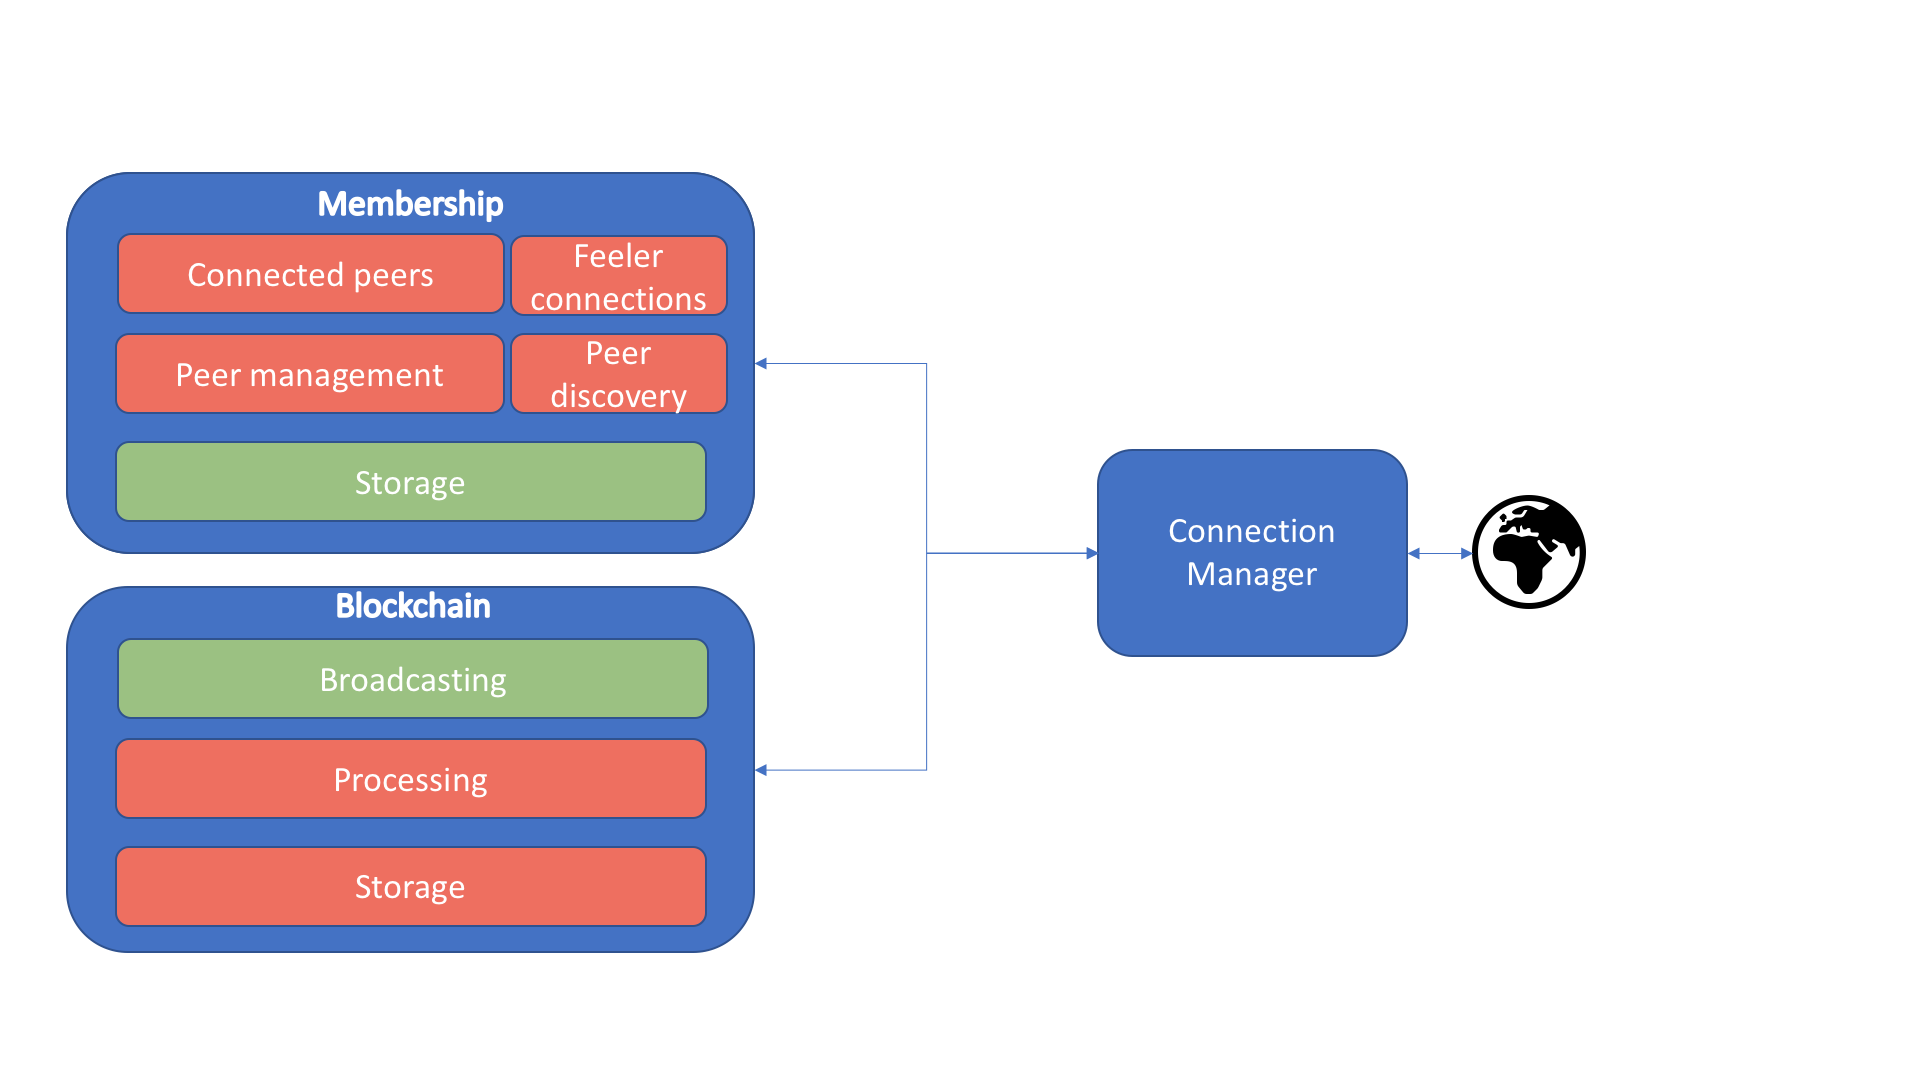
\includegraphics[scale=0.30]{figs/Architecture}
\caption{BitShield architecture}
\label{fig:bitshieldoverview}
\end{figure}

\textit{BitShield} is positioned between the \textit{Connection Manager} and the \textit{Peer Discovery} because those are the modules we have identified as the cause of the problems Bitcoin has.

In the rest of this section, we will cover each vulnerability individually and propose possible approaches that will help Bitcoin overcome these vulnerabilities.
In Section \ref{sec:evulne}, we will propose possible approaches to vulnerabilities that attackers can use to exploit Bitcoin. Whereas in Section \ref{sec:ivulne}, we will propose possible strategies to cope with behaviours that nodes inside the network might have to exploit Bitcoin and increase profit.
\subsection{External vulnerabilities}
\label{sec:evulne}

\paragraph*{\textbf{Information Eclipsing}}
Our approach to this problem is to implement the optimization in the propagation discussed in Section \ref{sec:ieclipsing}. To achieve this, when a node receives a block the verification of a block is split into two phases an initial difficulty check and a transaction validation. After the node validating that the block is valid through the first validation phase, the node would asynchronously broadcast \textit{inv} messages to his neighbours while performing the transaction validation. This will decrease the mean time it takes for a block to reach a node hence reducing the probability of forks happening. The drawback of this solution is that it only lowers the probability this problem happening.

%Our approach to this problem is to make the whole network aware of the existence of a fork. To achieve this, when a node received a block with the same height as the blockchain head, if that block was received soon after the node had received the current blockchain head then instead of not broadcasting it, the node would broadcast it allowing the full network to be aware of the fork. We believe this would lead to the end of the fork much faster. Because by making the full network aware of the fork nodes could choose which branch they would mine on.

It would also be interesting implementing the solution Ethereum used to solve this problem, \textit{Uncle Blocks} mentioned in Section \ref{sec:ieclipsing}. Where nodes include uncle blocks in future blocks strengthening the chain. They also reward nodes that found uncle blocks and nodes that add uncle blocks to their blocks which would compensate nodes that had their computational power wasted in a block that was not accepted. The problem with this approach is that it would have an increase in the block size and it would require more computational power from the nodes.

\paragraph*{\textbf{Partition attack}}
This attack is hard to protect against because the problem is not only related with Bitcoin but also with the protocol used by the ASes.

Hence, our aim is to use MACHETE and also make nodes establish some extra connections. In this approach, a node would have to establish extra connections while having into account the route that the packets were going to have then, nodes would also send certain key messages (like the \textit{inv} for instance) through multiple paths using the multipath approach of MACHETE. Nodes will use a tool like \textit{traceroute}\footnote{Diagnostic tool for displaying the route and measuring transit delays of packets across an Internet Protocol (IP) network.} to identify the best routes to avoid packets from passing always through the same AS. With this approach, a node is connected to the Bitcoin network through multiple AS and is able to communicate with different points of the network preventing the attack. A drawback of this approach would be the extra overweight imposed on the nodes to create the extra connections and send the extra messages.

\paragraph*{\textbf{Delay attack}}
This attack can be done in two different directions. Our approach is to address the problem in both directions as follows. Since this attack is targeted at a single connection that a node has with a neighbour of his. We will use a strategy like MACHETE and send multiple multiple block requests to different neighbours. With this strategy the attacker has to intercept more connections, this strategy also prevents the attack in both directions.

This solution might add overweight to the network because more request messages will be traversing the network. But if we compare the computational power wasted by the victim when being attacked with our solution, we believe that our solution will be better. Because not only are the messages small in size but also the victim will not be wasting computational power that could be used for strengthening the blockchain.

We also want to modify the behaviour of nodes in the \textit{N$\,\to\,$V} direction. Where once a node receives a corrupted block instead of staying idle it requests the block again. If the node fails 3 times to receive the block form that neighbour it drops the connection and asks for the block to another neighbour.

\paragraph*{\textbf{Mosquito attack}}
Our procedure to cope with this attack is to implement a system where every node analyzes the \textit{addr} messages that their neighbours share with them to identify if the neighbours are trying to attack them. The idea is if all neighbours are sharing the same set of addresses with a node through a period of time then the probability of them being malicious is high. If a node identifies a set of neighbours as malicious, he would ban those nodes and re-start its connection to the network. The disadvantages of this strategy are the extra computational power and memory wasted on the analysis of the \textit{addr} messages.

If we were to implement an approach where it costs a bit of the currency to send messages like Ripple or Ethereum. We would cope with this attack but it would require relevant changes to the Bitcoin protocol something that is not desirable by users in Bitcoin.

Implement authenticated messages for sharing IP addresses would also protect against the attack but it would require much more computational power and a system to distribute asymmetric key pairs.

\paragraph*{\textbf{51\% attack}}
For this attack, we are not going implement any solution in particular since this attack is always possible unless we control who joins the peer-to-peer network.

Still performing this attack in Bitcoin is very hard. Given the current competition in the mining community and the current size of the network, it would be very costly to gather 51\% of computational power.

\subsection{Internal vulnerabilities}
\label{sec:ivulne}
We will now address some of the solutions to the problems Bitcoin has with the behaviour of peers in the network and the way they connect between themselves.

\paragraph*{\textbf{Supernodes}}
To prevent this behaviour we are going to take advantage of the analysis that nodes are going to perform on \textit{addr} messages to prevent the mosquito attack. During the analysis, we will collect the number of times a node appears in those \textit{addr} messages and if a node reaches a certain number of appearances it is safe to presume that is a supernode. In this case, the node that identified the supernode will drop the connection with him and connect to another node. The disadvantages of this approach are once again the extra computational power required and also the possible increase of the mean time it takes for a block to propagate through all the network.

We could also introduce incentives towards a more random topology. An example of those incentives is the approach that Ripple and Ethereum used, where to send certain messages a node has to pay a fee. In our case to prevent supernodes, if a node exceeded a pre-established number of connections then for every extra connection the node would have to pay a fee in order to be able to sustain that connection. The problem with this approach is that we would have to modify the Bitcoin protocol something that is highly vetted against by the Bitcoin community.

\paragraph*{\textbf{Rational nodes}}
In Section \ref{sec:rpsummary}, we saw that in Bitcoin \textit{rational nodes} or \textit{selfish miners} do not behave like \textit{free riders} so we cannot implement directly approaches like the ones presented in before. In the context of file sharing, \textit{free riders} are nodes that would set their upload rate to low while having a high download rate. This is not applicable to Bitcoin because \textit{rational nodes} still work but they do not share the results of their work so that others waste their time and resources.

To prevent this we are going to implement a solution like LiFTinG \cite{guerraoui2010lifting} where nodes verify each other. In this solution, nodes analyze the messages their neighbours are broadcasting. The idea is for a node to analyze if a neighbour is broadcasting a new block right after receiving another block at the same height. If the neighbour did this a certain number of times then it would be safe to assume that that neighbour was a \textit{selfish node}. Nodes punish \textit{selfish nodes} by dropping the connection with them. The disadvantage of this solutions is the extra computational power required to perform these verifications and also the possibility of false positives.

Another possible approach that would minimize the impact of this behaviour is the implementations of uncle blocks. Because in this system node still gets rewarded for finding a block at the same height as the new blockchain head, up to a certain height difference.

\subsection{Summary}
Table \ref{fig:tabel2} summarizes the approaches we discussed above. As is possible to observe, there is no solution that fixes all the problems.

From Table \ref{fig:tabel2} there are some approaches that are not feasible to implement given the Bitcoin requirements for performance, those approaches are the \textit{encrypted messages} and \textit{authenticated messages}. Both approaches would require nodes to perform considerable more computations which would lower the profit of miners. Hence, these solutions would never be accepted by the Bitcoin community.

Other approaches like \textit{uncle blocks} and the \textit{implementation of fees} would be equally hard to implement given the relevant impact they would have on the protocol. Since \textit{uncle blocks} requires multiple nodes to be rewarded by the discovery of a new block and the \textit{implementation of fees} would require fees to be imposed on messages. Hence, both solutions would lower the profit of not only miners but also users and would be highly vetted against by the Bitcoin community.

However, there are still some approaches in Table \ref{fig:tabel2} that combined are able to cope with the multiple vulnerabilities while having a low impact on performance. Those approaches are the \textit{optimization in block propagation}, establishment of \textit{extra connections between nodes}, the use of \textit{MACHETE} to send messages through multiple paths, \textit{analysis of addr messagues} and the use of a \textit{LiFTinG approach} to cope with rational nodes. Although all these solutions combined will probably require more computational power from the nodes if we compare them with the approaches described before their impact is much lower.

% Please add the following required packages to your document preamble:
% \usepackage{graphicx}
\begin{table}[]
\centering
\resizebox{\textwidth}{!}{%
\begin{tabular}{l|c|c|c|c|c|c|c|c|c|c|}
\cline{2-11}
 & \begin{tabular}[c]{@{}l@{}}Uncle\\ Blocks\end{tabular} & \begin{tabular}[c]{@{}l@{}}Optimization\\ in block\\ validation\end{tabular} & \begin{tabular}[c]{@{}l@{}}Extra\\ connections\\ between\\ nodes\end{tabular} & MACHETE & \begin{tabular}[c]{@{}l@{}}Encrypted\\ messages\end{tabular} & \begin{tabular}[c]{@{}l@{}}Monitor\\ RTTs\end{tabular} & \begin{tabular}[c]{@{}l@{}}Analyze\\ addr\\ messages\end{tabular} & Fees & \begin{tabular}[c]{@{}l@{}}Authenticated\\ messages\end{tabular} & \begin{tabular}[c]{@{}l@{}}LiFTinG\\ approach\end{tabular} \\ \hline
\multicolumn{1}{|l|}{\begin{tabular}[c]{@{}l@{}}Information\\ Eclipsing\end{tabular}} & $\bigcirc$ & $\bigcirc$ &  &  &  &  &  &  &  &  \\ \hline
\multicolumn{1}{|l|}{\begin{tabular}[c]{@{}l@{}}Partition\\ Attack\end{tabular}} &  &  & $\bigcirc$ & $\checkmark$ & $\checkmark$ & $\bigcirc$ &  &  &  &  \\ \hline
\multicolumn{1}{|l|}{\begin{tabular}[c]{@{}l@{}}Delay\\ Attack\end{tabular}} &  &  & $\bigcirc$ & $\checkmark$ & $\checkmark$ & $\checkmark$ &  &  & $\bigcirc$ &  \\ \hline
\multicolumn{1}{|l|}{\begin{tabular}[c]{@{}l@{}}Mosquito\\ Attack\end{tabular}} &  &  &  &  &  &  & $\checkmark$ & $\checkmark$ & $\checkmark$ &  \\ \hline
\multicolumn{1}{|l|}{51\% Attack} & $\bigcirc$ & $\bigcirc$ & $\bigcirc$ &  &  &  &  & $\bigcirc$ &  &  \\ \hline
\multicolumn{1}{|l|}{Supernodes} &  &  &  &  &  &  & $\checkmark$ & $\checkmark$ &  &  \\ \hline
\multicolumn{1}{|l|}{\begin{tabular}[c]{@{}l@{}}Rational\\ nodes\end{tabular}} & $\bigcirc$ &  & $\bigcirc$ &  &  &  &  & $\bigcirc$ &  & $\checkmark$ \\ \hline
\end{tabular}%
}
\caption{Solutions to the problems. \\ $\checkmark$ - Protects against the problem \\ $\bigcirc$ - Helps protect against the problem}
\label{fig:tabel2}
\end{table}

\section{Melhorando a Propagação das Transacções}

Nesta secção propomos um conjunto de alterações ao mecanismo de propagação de transacções na Bitcoin com o objectivo o tornar mais eficiente, nomeadamente, de reduzir o número de anúncios redundantes que cada nó da rede recebe. A nossa proposta é fundamentada nas seguintes observações:

\begin{itemize}
\item Actualmente, os nós recebem em média $3.33$ anúncios para cada transacção (quando bastaria receberem no máximo um único para garantir a recepção da transacção).
\item A rede possui dois mecanismos complementares para propagar transacções: a troca de anúncios (usada antes da transacção estar inserida num bloco) e a troca de blocos (que implicitamente anunciam as transacções que lhe estão associadas).
\item Por razões históricas, o segundo mecanismo é mais eficiente, pois todas as transações em falta num nó são enviadas numa única mensagem (enquanto que o mecanismo de propagação epidémica inicial, obriga a troca de uma mensagem individual para cada transacção).
\item A rede Bitcoin não tem requisitos estritos de latência para a propagação das transações, uma vez que a taxa de geração de blocos é significativamente mais lenta que o processo de propagação epidémico (em média, é gerado um novo bloco a cada 10 minutos).
\item Os mineiros são uma fracção reduzida do número total de nós. Apesar de ser fundamental que as transacções sejam conhecidas pelo mineiros, o protocolo de disseminação não distingue os mineiros dos restantes nós.
\item No protocolo epidémico actualmente usado na Bitcoin, os anúncios são escalonados para serem propagados para todos os vizinhos que o nó conhece (cerca de 125).
Este valor é substancialmente maior do que o valor teórico dos protocolos de disseminação epidêmicos que sugere que, mesmo na presença de faltas, basta propagar informação para um número de vizinhos que é aproximadamente logarítmico com o tamanho da rede~\cite{epidemicDiss}. Para o tamanho atual da rede, que possuí cerca de $10~000$ nós bastaria portanto propagar para $ ln(10~000) \approx 10$ vizinhos.
\end{itemize}

O principal desafio é reduzir a quantidade de anúncios redundantes trocada na rede e, ao mesmo tempo, assegurar que as transações chegam aos nós mineiros.
A intuição da abordagem proposta é enviesar o processo de propagação na direcção dos mineiros mais produtivos na rede sem, no entanto, deixar de assegurar que a informação é também propagada por caminhos alternativos para os restantes nós e mineiros.
Isto é concretizado através de duas modificações ao protocolo.
A primeira consiste em adicionar um novo campo às mensagens que propagam os blocos que indica o número de saltos que o bloco dá na rede.
Isto permite que cada nó fique a saber a que distância está o mineiro que gerou esse bloco.
Esta informação é codificada num inteiro e portanto tem um impacto negligenciável no tamanho total do bloco que ronda 1 MB\@.
A segunda modificação consiste em identificar localmente, com o passar do tempo, qual o caminho para os mineiros mais próximos e enviar a propagação de anúncios preferencialmente por estes caminhos.
Note-se que a partir do momento em que uma transacção é incluída num bloco, o processo de propagação por troca epidémica de anúncios deixa de ser relevante.

%\subsection{Seriação dos Vizinhos}

%Como foi referido acima, a estratégia proposta para poupar largura de banda pressupõe que cada nó descobre quais os melhores caminhos para chegar aos mineiros mais próximos. Isto é conseguido seriando o vizinhos por um critério de proximidade aos mineiros. Os vizinhos mais perto dos mineiros ficam listados no topo da tabela e os mais afastados são seriados no fundo da tabela.

%Para obter esta classificação, cada nó mantém, para cada vizinho, três variáveis: \textit{n}, o número total de blocos que recebeu desse vizinho; \textit{k} a distância acumulada desses blocos até aos mineiros que o produziram; e finalmente \textit{a}, o número total de blocos recebidos.
%Para permitir actualizar \textit{k}, associamos ao processo de propagação de um novo bloco, um contador que regista quantos saltos o bloco deu na rede Bitcoin (este campo é incrementado sempre que um nó reencaminha o bloco). Com base nestas variáveis, a classificação dos vizinhos num determinado intervalo de tempo \textit{T} é feita de acordo com a seguinte fórmula (em que os valores de $k$, $a$ e $n$ são os acumulados no período $T$):

%\[ \mbox{class}^{T}= (\dfrac{k^{T}}{n^{T}} + a^{T}-n^{T}) \]

%Esta caracterização evita que nós com baixa capacidade de mineração que geram blocos muito esporadicamente, fiquem indefinidamente com uma boa classificação.
%Isto é relevante pois uma percentagem dos blocos é gerada por nós com baixa capacidade de mineração, que queremos evitar  aleatórios assim, se enviássemos as nossas transações sempre para esses nós elas poderiam demorar muito tempo até aparecerem em blocos podendo até ficarem perdidas.
%Desta forma, balanceamos não só os vizinhos que têm melhor rácio distancia aos mineiros/número de blocos providenciados, mas também conseguimos ter em conta o número total de blocos que esse vizinho nos forneceu relativamente ao número total de blocos recebidos.

%Uma vez que a classificação de cada um dos vizinhos se vai alterando ao longo do tempo, o valor usado para seriar os vizinhos é uma média deslizante da classificação instantânea acima referida, dada por:

%\[ \mbox{class}^t = (1-\alpha) \cdot \mbox{class}^{t-1}  + \alpha \cdot \mbox{class}^{T} \]

%O factor $\alpha$ existe para evitar que vizinhos de  mineiros que já tenham sido extremamente activos no passado mas que no tempo actual já não o são, permanecem para sempre no topo da tabela. Nas nossas experiências usamos $\alpha=0.3$ e \textit{T} é configurado como sendo um intervalo de 4 horas.

%Cada vez que um nó recebe um bloco de um vizinho, a classificação é atualizada conforme descrito no Algoritmo~\ref{alg:class}.
%<++> os seguintes passos vão acontecer de forma a mantermos uma lista com os $m$ vizinhos com menor valor de classificação:



%Na nossa solução, de forma a que um nó consiga determinar para qual dos seus vizinhos deve enviar transações vai somar o inteiro que indica o número de saltos que o bloco dá na rede a uma variável associada ao vizinho de quem recebeu o bloco. Esta variável vai ser depois dividida pelo número total de blocos recebidos através desse vizinho de modo a possamos associar um valor de proximidade ao mineiro a cada vizinho. Visto que o campo presente nas mensagem que propagam os blocos deve ser incrementado sempre que um nó envia o bloco para um dos seus vizinhos é evidente que os vizinhos com o menor valor de proximidade a mineiros vão ser os vizinhos que teoricamente estarão mais perto dos mineiros.

%\subsection{Propagação Enviesada}
%\label{sec:propagacao}
%Dado que o nosso objectivo é fazer com que as transações que conhecemos cheguem rapidamente aos mineiros podemos utilizar o mecanismo descrito na secção anterior para atingir este objectivo. Assim se estivéssemos perante uma rede onde todos os nós cumpriam com o protocolo e os caminhos fossem resilientes o suficiente poderíamos apenas enviar as transações que recebíamos para o nosso vizinho que tivesse menor valor de classificação e inevitavelmente essas transações seriam adicionadas a um bloco.

%No entanto, para além das falhas por paragem, temos de ter em conta que os nós podem manipular o $k$ enviado aos seus vizinhos, colocando-o a zero.
%Deste modo seriam erradamente priorizados e poderiam ficar em vantagem de duas maneiras: conhecer as transações mais cedo, e não propagar as transações recebidas.
%ara evitar este problema, além de disseminarmos as transações para os vizinhos com mais prioridade, enviamos também para um conjunto aleatório de vizinhos, conforme descrito no Algoritmo~\ref{alg:diss}. Desta forma asseguramos que as transações continuam a ser disseminadas pelo resto da rede mesmo que tenhamos como vizinho um nó malicioso.
%Desta forma sempre que um nó receber uma transação vai enviar esta para o conjunto de vizinhos com melhor classificação\textit{m} e vai concorrentemente enviar a transação para um conjunto de nós escolhidos ao acaso \textit{a} tal como descrito no algoritmo abaixo:



%O valor de \textit{pi} (Push inicial) indica se quando uma transação é gerada deve ser enviada apenas para \textit{m} e \textit{a} ou para todos os vizinhos.
%e \textit{a} enviar para todos os seus vizinhos.
%Desta forma os valores de \textit{tamanho\_m}, \textit{tamanho\_a} e \textit{pi} podem depois ser alterados para obtermos diferentes padrões de propagação.
%Na Secção~\ref{sec:calibracao} discutimos as diferentes configurações testadas.

%\subsection{Concretização}

%O nosso objectivo de longo prazo é vir a incluir uma versão da nosso algoritmo na distribuição do Bitcoin. No entanto, esse processo é moroso e requer evidências das vantagens da solução. Não sendo exequível fazer experiências com milhares de nós num ambiente real com uma versão alterada do cliente Bitcoin, tivemos de recorrer a simulação para avaliar o nosso algoritmo.

%Para criarmos uma simulador fiel ao cliente original, começámos por fazer alterações ao cliente da \textit{Bitcoin Core} (cliente mais usado) para recolhemos estatísticas em relação às mensagens trocadas pelos clientes que usam a distribuição por omissão. Desta forma alteramos o cliente para que este capturasse as seguintes informações:
%\begin{itemize}
%\item anúncios de transações;
%\item transações que recebidas;
%\item transações presentes em blocos compactos que o nó não possuía e tinha de pedir de forma a poder reconstruir o bloco.
%\end{itemize}
%Uma vez feitas as alterações lançamos o cliente numa zona da rede não protegida onde ficou ligado à rede Bitcoin durante um mês. Com as métricas que recolhemos ficamos com informação de referencia para poder calibrar o simulador.

%As simulações recorrem a simulador de eventos discreto, programado em Python,  que funciona por ciclos. Em cada ciclo os nós verificam se têm eventos para processar e, em caso afirmativo, executam o código que processa esse evento. Este código mimetiza o comportamento de um cliente Bitcoin (foram concretizadas duas versões, uma que tem o comportamento padrão e outra que corre as nossas modificações). Como resultado de processar um evento, um nó pode gerar novos eventos (que serão processados em ciclos futuros). Cada ciclo do simulador corresponde a um segundo de tempo real.

%Uma simulação começa com a criação de uma rede de nós que pode ser carregada de um ficheiro ou criada de raiz. Na rede criada, cada nó tem  8 vizinhos \textit{de escoamento} que são escolhidos aleatoriamente entre todos os nós. Mais nós podem ser adicionados a esta lista de vizinhança caso estabeleçam uma ligação com o nó ficando estes nós marcados como \textit{incidentes}, nunca podendo um nó estabelecer mais do que 125 conexões.
%São também escolhidos ao acaso um conjunto de mineiros que mantêm o rácio mineiros número de nós na rede.  De seguida o simulador cria uma lista com os nós que vão gerar transações em cada ciclo. Depois da rede estar criada a simulação começa, onde cada nó sequencialmente executa a função \textit{CICLO}, verificando se necessita de gerar transações, de gerar um bloco ou de enviar anúncios de transações aos seus vizinhos.

%\begin{itemize}
%\item No momento de criar uma transação, o nó de origem regista este evento um contador global que captura quantas transações já foram criadas no sistema, adiciona a transação à sua lista de transações conhecidas e coloca essa transação nas filas de anúncios a enviar aos seus vizinhos. Cada transação tem o tamanho de  700 bytes.
%\item No momento de criar um bloco, um nó determina qual será o ciclo em que o cripto puzzle será resolvido. Após correr esta função vai buscar à sua lista de transações \textit{pendentes} transações até encher o bloco (1428 transações) ou ficar sem transações  \textit{pendentes}. Finalmente vai criar o bloco, adicioná-lo à sua lista de blocos e anunciá-lo aos seus vizinhos.
%\item Cada nó mantém, para cada um dos seus vizinhos, uma lista de anúncios \textit{prontos} a enviar. Para enviar anúncios aos seus vizinhos, o nó começa por calcular, para cada vizinho, qual vai ser o próximo ciclo em que deve realizar a transmissão (a propagação dos anúncios é atrasada deliberadamente, para reduzir o tráfego de controlo). Quando esse instante chegar, retira um anúncio da lista de \textit{prontos}, verifica se o vizinho ainda não conhece esse anuncio e, caso ele não o conheça adiciona esse anuncio, a uma lista de anúncios a transmitir. Este processo é repetido até a lista de anúncios \textit{prontos} ficar vazia ou a lista de anúncios a enviar chegar ao tamanho limite de  35. No fim deste processo,  a lista de anúncios é enviada.
%\end{itemize}

%No simulador,  concretizámos o funcionamento das principais mensagens trocadas por nós após terem estabelecido ligações, essas mensagens são mensagens \textsl{Inv, GetHeaders, Headers, GetData, Block, CmpctBlock, GetBlockTX, BlockTX} e \textsl{TX} . Vamos agora explicar o  comportamento de um nó quando recebe cada uma destas mensagens.

%Quando um nó recebe uma mensagem de anúncios \textsl{INV}, vai percorrer todos os anúncios nessa mensagem e, para cada anúncio, realiza os seguintes passos:
%\begin{itemize}
%\item Verifica qual o tipo de anúncio (existem dois tipos de anúncios, os que anunciam blocos e os que anunciam transações);
%\item Atualiza o inventário do vizinho que enviou a mensagem, registando a informação anunciada;
%\item Verifica se já possui a informação anunciada. Caso não a possua, vai adicionar essa informação a uma lista de informação a pedir.
%\end{itemize}

%No depois de ter iterado por todos os anúncios, o nó envia uma mensagem de \textsl{GetHeaders} caso o anúncio tenha sido de blocos e envia uma mensagem \textit{GetData} caso o anúncio tenha sido de transações.

%Quando um nó recebe uma mensagem de pedido de informação \textsl{GetData, GetHeaders}, vai atualizar o inventário do vizinho que lhe enviou a mensagem e vai responder com a informação requisitada.

%Quando um nó recebe uma mensagem de \textsl{Headers}, o nó itera sobre todos os cabeçalhos incluídos e adiciona-os à sua cadeia de cabeçalhos. Caso não conheça o antecessor de um bloco, o nó requisita também o cabeçalho respectivo. Depois de adicionar os cabeçalhos à cadeia de cabeçalhos, requisita os blocos associados a esses cabeçalhos com uma mensagem \textsl{GetData}.

%Quando um nó recebe uma mensagem de \textsl{TX}, vai atualizar o inventário do vizinho e seguidamente caso não possua a transação, adiciona-a à sua lista de transacções \textit{pendentes} e invoca uma função, designada por \textit{push\_to\_send}, para disseminar essa transação aos vizinhos que ainda não a possuem.

%Quando um nó recebe um bloco compacto através de uma mensagem \textsl{CmpctBlock}, o nó verifica se já possui esse bloco e caso já o possua  atualiza apenas o inventário do vizinho que lhe enviou o bloco. Caso não possua o bloco, verifica se têm todas as transações presentes no bloco;  se não possuir uma ou mais transações requisita-as com uma mensagem de \textsl{GetBlockTX} e coloca o bloco numa lista de blocos parcialmente construidos. Assim que receber a resposta à mensagem de requisito de transações acaba de reconstruir o bloco e inicia o processamento do novo bloco. Quando um nó recebe um bloco completo através de uma mensagem \textsl{Block}, caso não o possua vai processá-lo.

%O processamento de um bloco começa por atualizar o inventário de blocos. Caso o novo bloco seja posterior ao bloco mais recente que o nó conhece, atualiza-se o estado do livro razão dá-se inicio ao cálculo de um novo bloco. Por fim,  antes de se iniciar a disseminação do bloco,  removem-se as transações incluídas no bloco da lista de transações \textit{pendentes}. Durante a disseminação de um bloco, se o vizinho possuir o bloco anterior ao novo bloco então envia-se o novo bloco através de uma mensagem \textsl{CmpctBlock}; caso contrário envia-se uma mensagem de \textsl{Header}.

%A versão modificada, que suporta o nosso algoritmo, executa a seguinte funcionalidade adicional. Em primeiro lugar, é associado ao processo de propagação de um novo bloco, um contador que regista quantos saltos o bloco deu na rede Bitcoin até chegar ao nó que o está a receber. Isto permite que cada nó mantenha uma estimativa da sua distância, em número de saltos, para cada mineiro e quais os vizinhos que fazem parte do caminho para esses mineiros. Como os blocos não percorrem sempre o mesmo percurso, esta distância poderá variar cada vez que um bloco é produzido, pelo que cada nó vai mantendo uma média deslizante desta distância, que é actualizada sempre que chega um novo bloco. Cada nó mantém também informação de quantos blocos foram gerados por cada mineiro. Estas duas informações permitem estabelecer uma ordenação dos vizinhos, em que os vizinhos mais perto dos mineiros mais produtivos são seriados no topo da tabela, e os vizinhos afastados desses mineiros são relegados para o fim da tabela. Esta seriação é posteriormente usada para enviesar o processo de propagação de transacções: sempre que um nó executar a função \textit{push\_to\_send} para anunciar novas transações, vai apenas adicionar a transacção à lista anúncios \textit{pendentes} de alguns dos vizinhos, de acordo com o algoritmo descrito anteriormente.

\chapter{Evaluation}
\section{Evaluation}
\label{sec:evaluation}
Given how adverse the Bitcoin community is to change once we evaluate our system we will have to take into account the following factors that are a priority for both Bitcoin users and miners.

\begin{itemize}
\item \textbf{Transaction and block latency} As it was described in the previous section, some of the approaches have an impact on the time it takes to disseminate transactions or blocks. So once we evaluate our system we will have to study if our system does not increase this latency time by a relevant amount. Otherwise, our system might induce more forks on the network which is not desirable.

\item \textbf{Bandwith consumption} This factor is also important for two reasons: i) we want to preserve computational power and ii) we want our system to be scalable. 

We want to minimize the number of messages on the network to avoid nodes from wasting computational power processing irrelevant messages. Furthermore, with the growing number of Bitcoin users if our system was to put a big overweight on the network it would not scale well. 

Some of our approaches will impose an extra overweight on the network so once we evaluate our system we will have to take into consideration that extra bandwidth and try to minimize it.

\item \textbf{Resources consumption} This is one of the most important factors given the performance requirements imposed by the Bitcoin community. If our system was to downgrade the performance of Bitcoin without a worthy tradeoff our system would never be adopted. It is certain that with the implementation of our approaches the performance aspect of Bitcoin will be affected. So once we evaluate our system we will need to take this into consideration and balance out the performance degradation with the advantages our system brings.
\end{itemize}

Given the complexity of Bitcoin and its dimension we will start by using the Shadow simulator \cite{jansen2011shadow} to evaluate our system. We will use an incremental approach to test our system given the complex system that Bitcoin is. We will start by examining if each our approaches protect Bitcoin against their respective vulnerabilities. Then once we are sure that our strategies work as expected we will combine them together and once again evaluate their effectiveness and also measure the factors presented previously. 

Our system should be tested with a workload that contains the same amount of transactions happening these days but the amount of messages should be proportional to the size of the emulated network, for instance, we are not going emulate a system with 10 nodes and 100K transactions.

Finally, once we have a good understanding of the impact Bitshield has in Bitcoin we will generate, if there is still enough time until the deadline of the thesis, a working Bitcoin client ready to be deployed in the network.

Para avaliar a abordagem proposta, construímos um simulador de eventos que modela a propagação de transações na rede Bitcoin (este simulador foi desenvolvido em Python). Decidimos implementar o nosso próprio simulador pois todos os outros que encontrámos não implementavam a versão mais actual do protocolo Bitcoin\footnote{Entre outros \url{https://github.com/shadow/shadow-plugin-bitcoin} e\\ \url{https://github.com/arthurgervais/Bitcoin-Simulator}}. 

\subsection{Calibração do Simulador}
\label{sec:calibracao}
De modo a calibrar o simulador para ser o mais fiel possível ao protocolo original, extendemos o \textit{Bitcoin Core}, o cliente Bitcoin mais usado, para recolher métricas relativamente às mensagens trocadas pelos clientes.
As métricas recolhidas são as seguintes: i) anúncios de transações; ii) transações recebidas; iii) transações presentes em blocos compactos que o nó não possuía e tinha de pedir de forma a poder reconstruir o bloco.
Corremos duas instâncias deste cliente, em localizações físicas distintas durante um mês e usámos as métricas recolhidas para calibrar e validar o simulador.
Além disso usámos a informação publicamente disponível em \url{https://blockchain.info/} para determinar o número de transações criadas por dia, a distribuição de blocos gerados por mineiro, e o tamanho médio de uma transação.
Munidos destas métricas, implementámos o protocolo original no simulador, bem como as nossas modificações. Calibrámos experimentalmente o simulador de modo a que os resultados observados no Bitcoin fossem equivalentes às observações efetuadas no cliente real.
O modelo de rede que usámos para as simulações foi composto apenas por nós que seguem o protocolo devidamente.

%As simulações recorrem a simulador de eventos discreto, programado em Python,  que funciona por ciclos. Em cada ciclo os nós verificam se têm eventos para processar e, em caso afirmativo, executam o código que processa esse evento. Este código mimetiza o comportamento de um cliente Bitcoin (foram concretizadas duas versões, uma que tem o comportamento padrão e outra que corre as nossas modificações). Como resultado de processar um evento, um nó pode gerar novos eventos (que serão processados em ciclos futuros). Cada ciclo do simulador corresponde a um segundo de tempo real.




%Para testar a nossa solução corremos o nosso simulador em diferentes maquinas para diferentes tamanhos de rede. Para realizar a maior partes dos testes usamos um computador pessoal com um Intel i5-4590 e 12GB de RAM usamos também para correr testes de maior dimensão uma maquina com um AMD Opteron 6272 e 32GB de RAM e outra maquina com um XX e 125GB de RAM.


%Dados serem computacionalmente dispendiosas, as simulações foram corridas para diferentes tamanhos de rede mantendo o rácio de mineiros observado na data de realização das experiências, 6000 nós para 16 pools de mineiros cada uma com 3 gateways em média. Assim os diferentes tamanhos de rede testados foram: 625 nós com 5 mineiros, 1000 nós com 12 mineiros e 6000 nós com 48 mineiros todos para uma duração equivalente a um dia em tempo real.
Devido às simulações serem computacionalmente dispendiosas e demorarem muito tempo a correr (na ordem dos dias) para redes grandes, fizemos testes preliminares para verificarmos se podíamos diminuir proporcionalmente o tamanho da rede e respectivas propriedades sem comprometer os resultados obtidos.
Para este efeito, corremos o protocolo original com 6000 nós e com 625 nós e comparámos várias métricas, que discutiremos mais adiante.
Os resultados obtidos foram equivalentes para ambos os tamanhos de rede pelo que, no resto desta secção consideramos uma rede de 625 nós.
Este escalonamento proporcional entre 6000 nós (tamanho de rede registado quando começamos as experiências) e 625 nós permitiu-nos explorar mais rapidamente o espaço de soluções e correr várias instâncias de cada teste.
Os resultados apresentados são a média de 3 testes independentes e correspondem a 24 horas de tempo real.

%e 16 \emph{pools} de mineiros cada uma com 3 \gateways em média quer com uma rede de 625 nós e 5 pools cada uma com 1 gateway. Assim todos os nossos testes foram realizados para uma duração equivalente a um dia em tempo real com a configuração para os 625 nós.
%no mundo real o que significa 86400 ciclos no simulador.

 
%De forma a podermos correr múltiplas simulações de uma só vez escrevemos também um \textit{script} em Bash que nos permitia correr as diferentes experiências múltiplas vezes e até paralelamente caso o máquina em questão tivesse recursos suficientes para o fazer. 

\subsection{Impacto da Propagação Enviesada}
\label{sec:evalDiss}
Começámos por explorar o espaço de soluções à procura de compromissos que nos permitam reduzir o consumo de recursos de rede sem ter um impacto negativo nas propriedades dos sistema.
Para ser mais fácil denominar as diferentes experiências realizadas usamos a seguinte notação: \textsl{Mn}, em que n especifica o valor da variável \textsl{tamanho\_m} ; e \textsl{An}, em que n especifica o tamanho da variável \textsl{tamanho\_a} conforme especificado no Algoritmo~\ref{alg:diss}.

%\begin{itemize}
%\item Top n - tamanho da lista de melhores nós;
%\item Rand n - tamanho do conjunto de nós escolhidos ao acaso.
%\end{itemize}

Inicialmente, testámos as combinações de $n={1,2,3,4}$ quer para \textsl{M} quer para \textsl{A}.
Após este conjunto preliminar de experiências, observámos que os resultados para $n={3,4}$ eram praticamente indistinguíveis de $n={1,2}$, com a excepção do número de duplicados que permaneceu perto do obtido na Bitcoin original.
Estes resultados suportam também as medições no cliente real, onde observámos um número médio de duplicados de $3.33$. 
Deste modo, para o resto das experiências efectuadas, consideramos somente as combinações:
%Inicialmente para que pudesse-mos  averiguar a eficácia da nossa solução começamos por correr um conjunto de experiências com n igual a 4, 3, 2, 1 quer para Top quer para Rand. 
%
%Dos resultados destas experiências pudemos concluir que os valores de n a 4 e 3 ainda eram muito elevados pois obtínhamos os mesmo resultados que com n igual a 2 e 1 só que tínhamos uma percentagem de mensagens de anúncios duplicadas ainda muito próxima à versão base. Desta forma decidimos correr os testes para as seguintes combinações:
%\begin{itemize}
M2\_A2;
M2\_A1;
M2\_A0;
M1\_A1;
M1\_A0.
%\end{itemize}
%\textbf{MM: TODO: esta parte deveria esta na especificação acima.}
Adicionalmente, para cada configuração variámos o valor da variável \textsl{pi}.
%Após termos corrido algumas experiências tivemos a ideia de também adicionar um mecanismo a que chamámos \textit{Early push}, que consiste num nó quando cria uma transação em vez de enviar só para o Top e os Rand envia para todos os seus vizinhos. Assim as experiências que vamos observar têm as 5 diferentes combinações e para cada uma ainda mostramos os resultados com o \textit{Early push} ativado e desativado. 
Nos dados apresentados abaixo descartámos também a primeira e a última hora de simulação de forma a podermos estudar o sistema em estado estável.
\vspace{-0.7cm}

\begin{figure}
\centering
%\begin{subfigure}{.45\textwidth}
%  	\centering
%	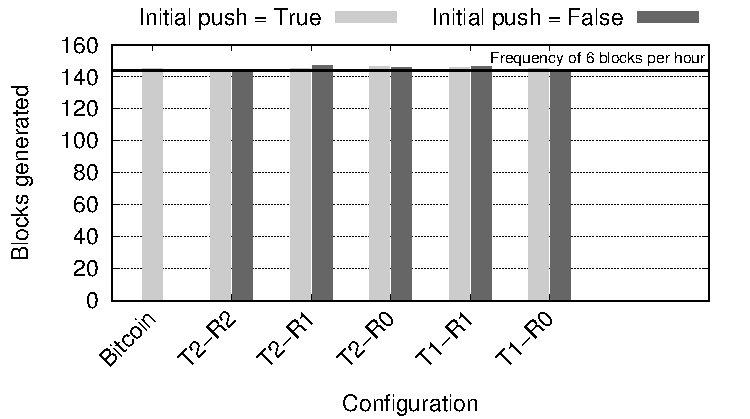
\includegraphics[width=1\textwidth]{plots/blocks-gen.pdf}
\subfloat[Quantidade de blocos criados.]{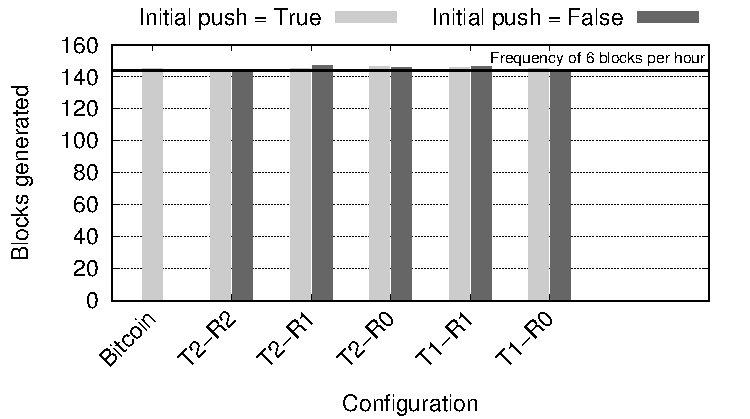
\includegraphics[width=0.45\textwidth]{plots/blocks-gen.pdf}
%	\caption{Quantidade de blocos criados}
	\label{fig:nb-blocks}
}
%\end{subfigure}%
%\begin{subfigure}{.5\textwidth}
%	\centering
\subfloat[Percentagem de transações adicionadas aos blocos.]{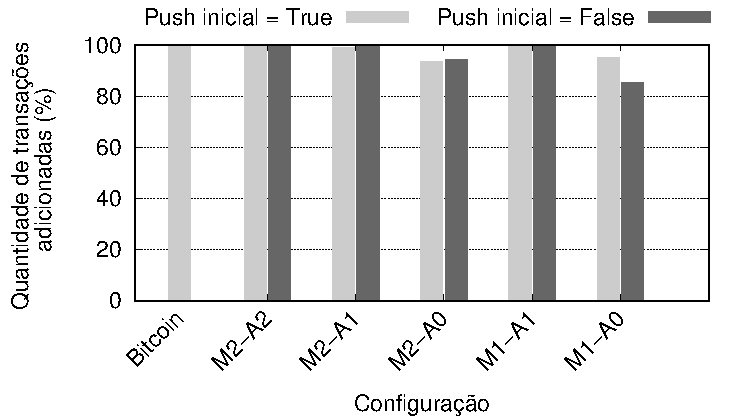
\includegraphics[width=.45\textwidth]{plots/tx-added.pdf}
	\label{fig:tx-added}
}
\caption{Blocos criados e percentagem de transações adicionadas aos blocos nos diferentes cenários considerados.}
%\end{subfigure}
\vspace{-0.7cm}
\end{figure}

A Figura~\ref{fig:nb-blocks} apresenta, para cada configurações a quantidade de blocos que foi gerada ao longo da experiência, enquanto que a Figura~\ref{fig:tx-added} mostra a percentagem de transações que foram adicionadas aos blocos. 
%No eixo do x temos as diferentes configurações e no eixo do y temos a percentagem de transações adicionada.
Para o cenário Bitcoin obtemos o número esperado de blocos num dia ($\approx 144$) bem como o número de transações incluídas nos blocos ($\approx 100\%$).
Todas as configurações produzem aproximadamente o mesmo número de blocos, contudo para as configurações M2\_A0 e M1\_A0 nem todas as transações são incluídas nos blocos.
Na prática isto quer dizer que nem todas as transações chegam a todos os mineiros, e ilustra a importância de manter a aleatoriedade da disseminação.

%Ambas as figuras mostram que o nosso simulador é capaz de simular com alguma fidelidade a Bitcoin pois podemos observar na coluna do Bitcoin que quantidade de blocos gerados está bastante próximo dos seis blocos à hora e que todas as transações geradas durante a simulação foram incluídas em blocos. 
Na Figura~\ref{fig:commit-time} estudamos o tempo médio desde que uma transação é criada até ser incluída num bloco. As linhas horizontais denotam o tempo médio para uma transação ser incluída num bloco no Bitcoin. 
%As linhas horizontais denotam o tempo médio de uma transação na coluna Bitcoin encontra-se dentro dos limites esperados.
Mais uma vez, a aleatoriedade ajuda não só a a que as transações cheguem a todos os nós como também diminui consideravelmente o tempo necessário para as transações serem incluídas nos blocos.
\vspace{-0.6cm}

\begin{figure}
\centering
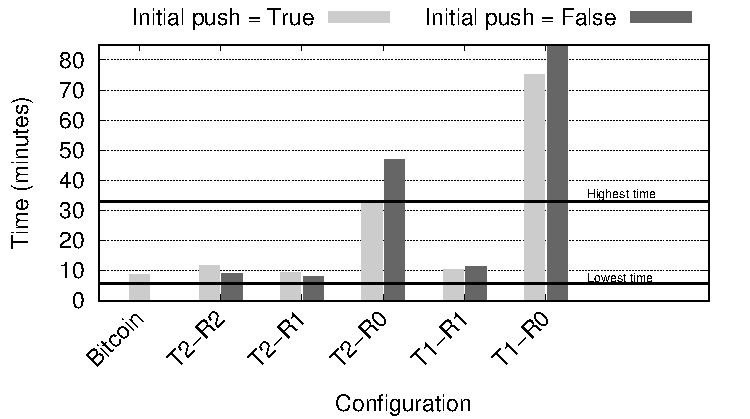
\includegraphics[width=0.8\textwidth]{plots/commit-time.pdf}
\caption{Tempo médio que demora desde que uma transação é criada até ser incluída num bloco.}
%Para as configurações em que nem todas as transações são incluídas, ignoramos essas transações.}	
\label{fig:commit-time}
\vspace{-1.5cm}
\end{figure}

%\subsection{Desempenho}

\begin{figure}
\centering
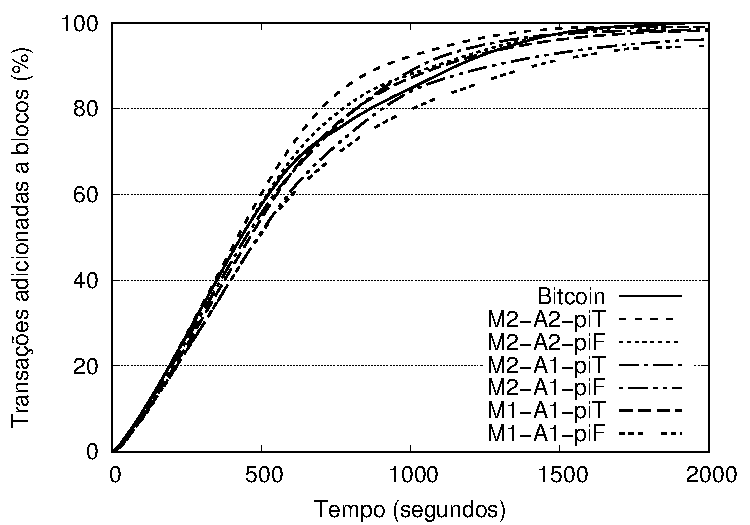
\includegraphics[width=0.6\textwidth]{plots/cdf_commit_2000.pdf}
\caption{Função de distribuição acumulada do tempo necessário para uma transação ser incluída num bloco.}
%CDF do tempo de commit. Nesta figura não mostramos no eixo do \textsl{x} todas as configurações a atingir as 100\% transações adicionadas pois se o fizéssemos a figura tornar-se-ia ilegível.}
\label{fig:cdf-commit}
\vspace{-0.5cm}
\end{figure}

A Figura~\ref{fig:cdf-commit} apresenta a função de distribuição acumulada do tempo necessário para incluir transações num bloco, sendo portanto uma perspectiva diferente da Figura~\ref{fig:commit-time}.
Curiosamente, enviar a transação a primeira vez para todos os vizinhos (\emph{pi=T}) tem um impacto residual no tempo que as transações demoram a ser incluídas no bloco.
Isto deve-se ao facto de a taxa de criação de blocos ser bastante reduzida face ao tempo de propagação fim-a-fim da rede.
%, permitindo assim poupanças adicionais.
%a CDF do tempo de commit. Nesta figura podemos observar que existem configurações onde grande parte das transações demora mais de 166 minutos a serem adicionadas aos blocos, isto acontece especialmente nas configurações M2\_A0 e M1\_ A0. Daqui conseguimos concluir que estas configurações não são muito viáveis.

\begin{figure}
\centering
\begin{minipage}{.5\textwidth}
  	\centering
  	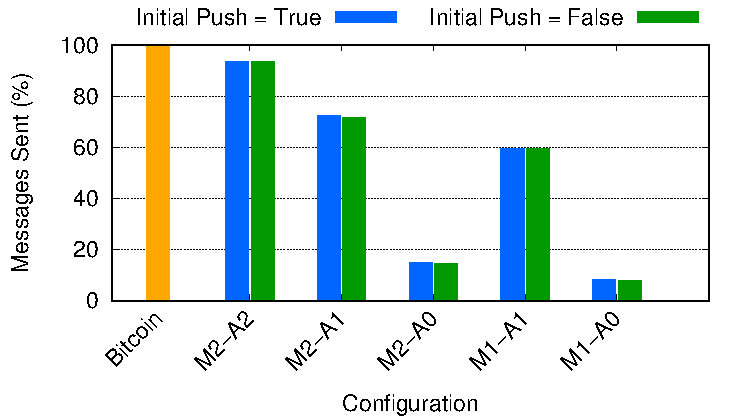
\includegraphics[width=1\textwidth]{plots/msg-sent.pdf}
	\caption{Numero total de mensagens \\\hspace{\textwidth} enviadas.}
	\label{fig:msg-sent}
\end{minipage}%
\begin{minipage}{.5\textwidth}
  	\centering
  	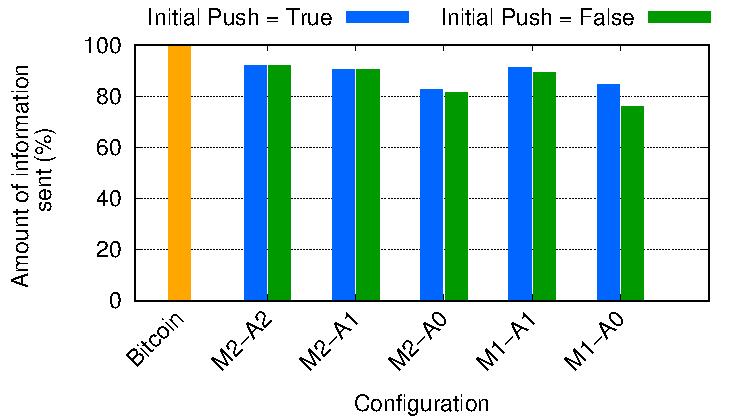
\includegraphics[width=1\textwidth]{plots/mb-sent.pdf}
	\caption{Quantidade de informação \\\hspace{\textwidth} enviada.}
	\label{fig:mb-sent}
\end{minipage}
\vspace{-0.5cm}
\end{figure}

Analisado o impacto nos efeitos observáveis da rede, nomeadamente o tempo que uma transação demora a ser incluída num bloco e a quantidade de transações incluídas, focamo-nos agora no ganhos, em termos de mensagens poupadas e redução da quantidade de informação transmitida.


A Figura~\ref{fig:msg-sent} mostra o número total de mensagens que foram enviadas em percentagem das enviadas na rede Bitcoin.
%No eixo do \textit{x} temos as diferentes configurações e no eixo do \textit{y} a percentagem de mensagens enviadas em relação à versão Bitcoin.
Como esperado, as configurações com mais poupanças são as que não enviam transações para nós aleatórios, pois é provável que esses nós não tenham a transação e logo irão pedi-la ao emissor.
%isto porque ao enviar anúncios de transações para nós A vamos quase de certeza receber um pedido para a transação que anunciamos pois muito provavelmente eles ainda não têm a transação, o mesmo já não acontece quando se envia transações para nós M.
No entanto, como vimos anteriormente, estas configurações não são viáveis pois nem todas as transações são incluídas e, as que são, tendem a demorar bastante tempo.
A Figura~\ref{fig:mb-sent} mostra a quantidade de informação total enviada em percentagem que, como esperado, segue uma tendência semelhante à Figura~\ref{fig:msg-sent}.
Podemos observar que a poupança em quantidade de informação enviada não é tão significativa como a das mensagens, pois as mensagens de anúncio são pequenas.
No entanto, na prática, processar essas mensagens desnecessariamente impõe um custo nos nós.
%todos os nós vão ter sempre que acabar por receber as transações, desta forma só conseguimos poupar nos anúncios destas. No entanto entre as duas configurações de M1\_A1 podemos ver que com o push inicial a False vamos obter a maior poupança.

Analisando estes resultados, é possível concluir que a configuração mais atrativa é M1\_A1 com \textsl{pi=F} pois obtém bons ganhos 
(redução da quantidade de mensagens em 40.5\% e  redução total da quantidade de informação enviada em 10.7\%) ao mesmo tempo que preserva as propriedades da Bitcoin original.


\chapter{Conclusions}
\label{chap:conclusions}
Despite the multiple iterations and improvements  that have been done to the Bitcoin dissemination protocol since its introduction, there are still  some aspects that need to be improved.
As Bitcoin becomes more popular and new clients join the system, it is fundamental to have an efficient and robust dissemination substrate for the network to function properly.
%Given the current size of the network and the introduction of new clients to the system is of utmost importance that the new systems are efficient without hurting the resilience of the system.
In this paper, we took some steps in this direction by improving the existing algorithm to do a more selective dissemination.
Our improvements allow to save, 10.2\% of the current bandwidth used and 41.5\% of the number of messages exchanged without compromising the robustness of the current approach.

As future work, we plan to leverage more detailed membership information to build more efficient dissemination paths.



\bibliographystyle{chicago}
\bibliography{references}
\addcontentsline{toc}{chapter}{{\small Bibliography}}


\end{document}
